%\documentclass[xcolor=table,handout,compress]{beamer}
\documentclass[xcolor=table]{beamer}
%--------------------------------------------------------------------------
% Common packages
%--------------------------------------------------------------------------
\usepackage[english]{babel}
\usepackage{pgfpages} % required for notes on second screen
\usepackage{graphicx}
\usepackage{subfigure}
\usepackage{multicol}
\usepackage[normalem]{ulem}

\usepackage{tabularx,ragged2e}
\usepackage{booktabs}
\usepackage{marvosym}

\makeatletter
\let\beamer@writeslidentry@miniframeson=\beamer@writeslidentry
\def\beamer@writeslidentry@miniframesoff{%
  \expandafter\beamer@ifempty\expandafter{\beamer@framestartpage}{}% does not happen normally
  {%else
    % removed \addtocontents commands
    \clearpage\beamer@notesactions%
  }
}
\newcommand*{\miniframeson}{\let\beamer@writeslidentry=\beamer@writeslidentry@miniframeson}
\newcommand*{\miniframesoff}{\let\beamer@writeslidentry=\beamer@writeslidentry@miniframesoff}
\makeatother


%--------------------------------------------------------------------------
% Load theme
%--------------------------------------------------------------------------
\usetheme{hri}

\usepackage{tikz}
\usetikzlibrary{patterns,shapes,fpu,fit,calc,mindmap,backgrounds,positioning,svg.path}

\tikzset{
  invisible/.style={opacity=0},
  visible on/.style={alt={#1{}{invisible}}},
  alt/.code args={<#1>#2#3}{%
    \alt<#1>{\pgfkeysalso{#2}}{\pgfkeysalso{#3}} % \pgfkeysalso doesn't change the path
  },
}

%% Neat trick to have only one navigation bullet per subsection
%% http://tex.stackexchange.com/questions/64333/one-navigation-bullet-per-subsection-with-subsection-false-in-custom-beamer-them
%\usepackage{etoolbox}
%\makeatletter
%\patchcmd{\slideentry}{\advance\beamer@xpos by1\relax}{}{}{}
%\def\beamer@subsectionentry#1#2#3#4#5{\advance\beamer@xpos by1\relax}%
%\makeatother
%%%%%%%%%%%%%%%%%%%%%%%%%%%%%%%%%%%%%%%

\graphicspath{{figs/}}

% for model of anthopomorphism
\newcommand{\IPA}{{$\mathcal{A}_0$~}}
\newcommand{\SLA}{{$\mathcal{A}_\infty$~}}
\newcommand{\sla}{{\mathcal{A}_\infty}}
\newcommand{\AntMax}{{$\mathcal{A}_{max}$~}}
\newcommand{\antMax}{{\mathcal{A}_{max}}}

% for HATP plans
\newcommand{\hatpaction}[3]{#1\\\textsf{\scriptsize #2,}\\\textsf{\scriptsize #3}}
\newcommand{\stmt}[1]{{\footnotesize \tt  #1}}

% for mutual modelling
\newcommand{\Mmodel}[3]{{\mathcal{M}(#1, #2, #3)}}
\newcommand{\model}[3]{{$\mathcal{M}(#1, #2, #3)$}}
\newcommand{\Model}[3]{{$\mathcal{M}^{\circ}(#1, #2, #3)$}}

% typeset logical concept
\newcommand{\concept}[1]{{\scriptsize \texttt{#1}}}

\newcommand{\backbutton}{\hfill\hyperlink{appendix}{\beamerreturnbutton{Supplementary material}}}
%--------------------------------------------------------------------------
% General presentation settings
%--------------------------------------------------------------------------
\title{\Large Socially-driven Autonomous Robots\newline for Real-World Human-Robot Interactions}
\subtitle{~}
\date{ISIR -- {\bf 06 Jan 2021}}
\author{Séverin Lemaignan}
\institute{Bristol Robotics Lab\\{\bf University of the West of England}}

%--------------------------------------------------------------------------
% Notes settings
%--------------------------------------------------------------------------
%\setbeameroption{show notes on second screen}
%\setbeameroption{hide notes}

\begin{document}


%%%%%%%%%%%%%%%%%%%%%%%%%%%%%%%%%%%%%%%%%%%%%%%%%%%%%%%%


%%%%%%%%%%%%%%%%%%%%%%%%%%%%%%%%%%%%%%%%%%%%%%%%%%%%%%%%

%\maketitle
\imageframe{titlepage}

%%%%%%%%%%%%%%%%%%%%%%%%%%%%%%%%%%%%%%%%%%%%%%%%%%%%%%%%

\section*{Bio}


{\fullbackground{europe_map}
\begin{frame}{SHORT BIO}

    \begin{columns}
        \begin{column}{0.7\linewidth}

    \begin{itemize}
        \item \textbf{2008--2012} Joint French (LAAS-CNRS) German (TU
            Munich) PhD\\
            \begin{itemize}
                \item AI \& Cognitive Robotics
                \item Prix GdR Meilleure thèse
            \end{itemize}

        \item \textbf{2013--2015} Post-doc at EPFL
            \begin{itemize}
                \item Creation of the HRI team
                \item Two main projects: \emph{CoWriter} \& \emph{Cellulo}
            \end{itemize}

        \item \textbf{2015-2018} Post-doc at Plymouth University, UK
            \begin{itemize}
                \item EU Marie Curie fellowship
                \item Social Cognition in Robotics
            \end{itemize}

        \item \textbf{2018--} Associate Prof. at Bristol Robotics Lab

    \end{itemize}

    \end{column}
        \begin{column}{0.4\linewidth}
    \end{column}
    \end{columns}
            
\end{frame}
}

%\imageframe[color=black]{perso/robots}

\imageframe{my_background/00}

%%%%%%%%%%%%%%%%%%%%%%%%%%%%%%%%%%%%%%%%%%%%%%%%%%%%%%%%

\section*{Academic background}

{
    \paper{Lemaignan et al. \textbf{Grounding the Interaction: Anchoring Situated Discourse in Everyday [...]} Intl. Journal of
    Social Rob. 2011]\\

    [Lemaignan et al. \textbf{Artificial Cognition for Social Human-Robot
    Interaction: An Implementation} Artificial Intelligence 2017}

    \begin{frame}<4>[label=sitass]{SYMBOLIC SOCIAL COGNITION FOR REAL-WORLD
        AUTONOMY}

        \begin{columns}
            \begin{column}{0.3\linewidth}
                \centering
                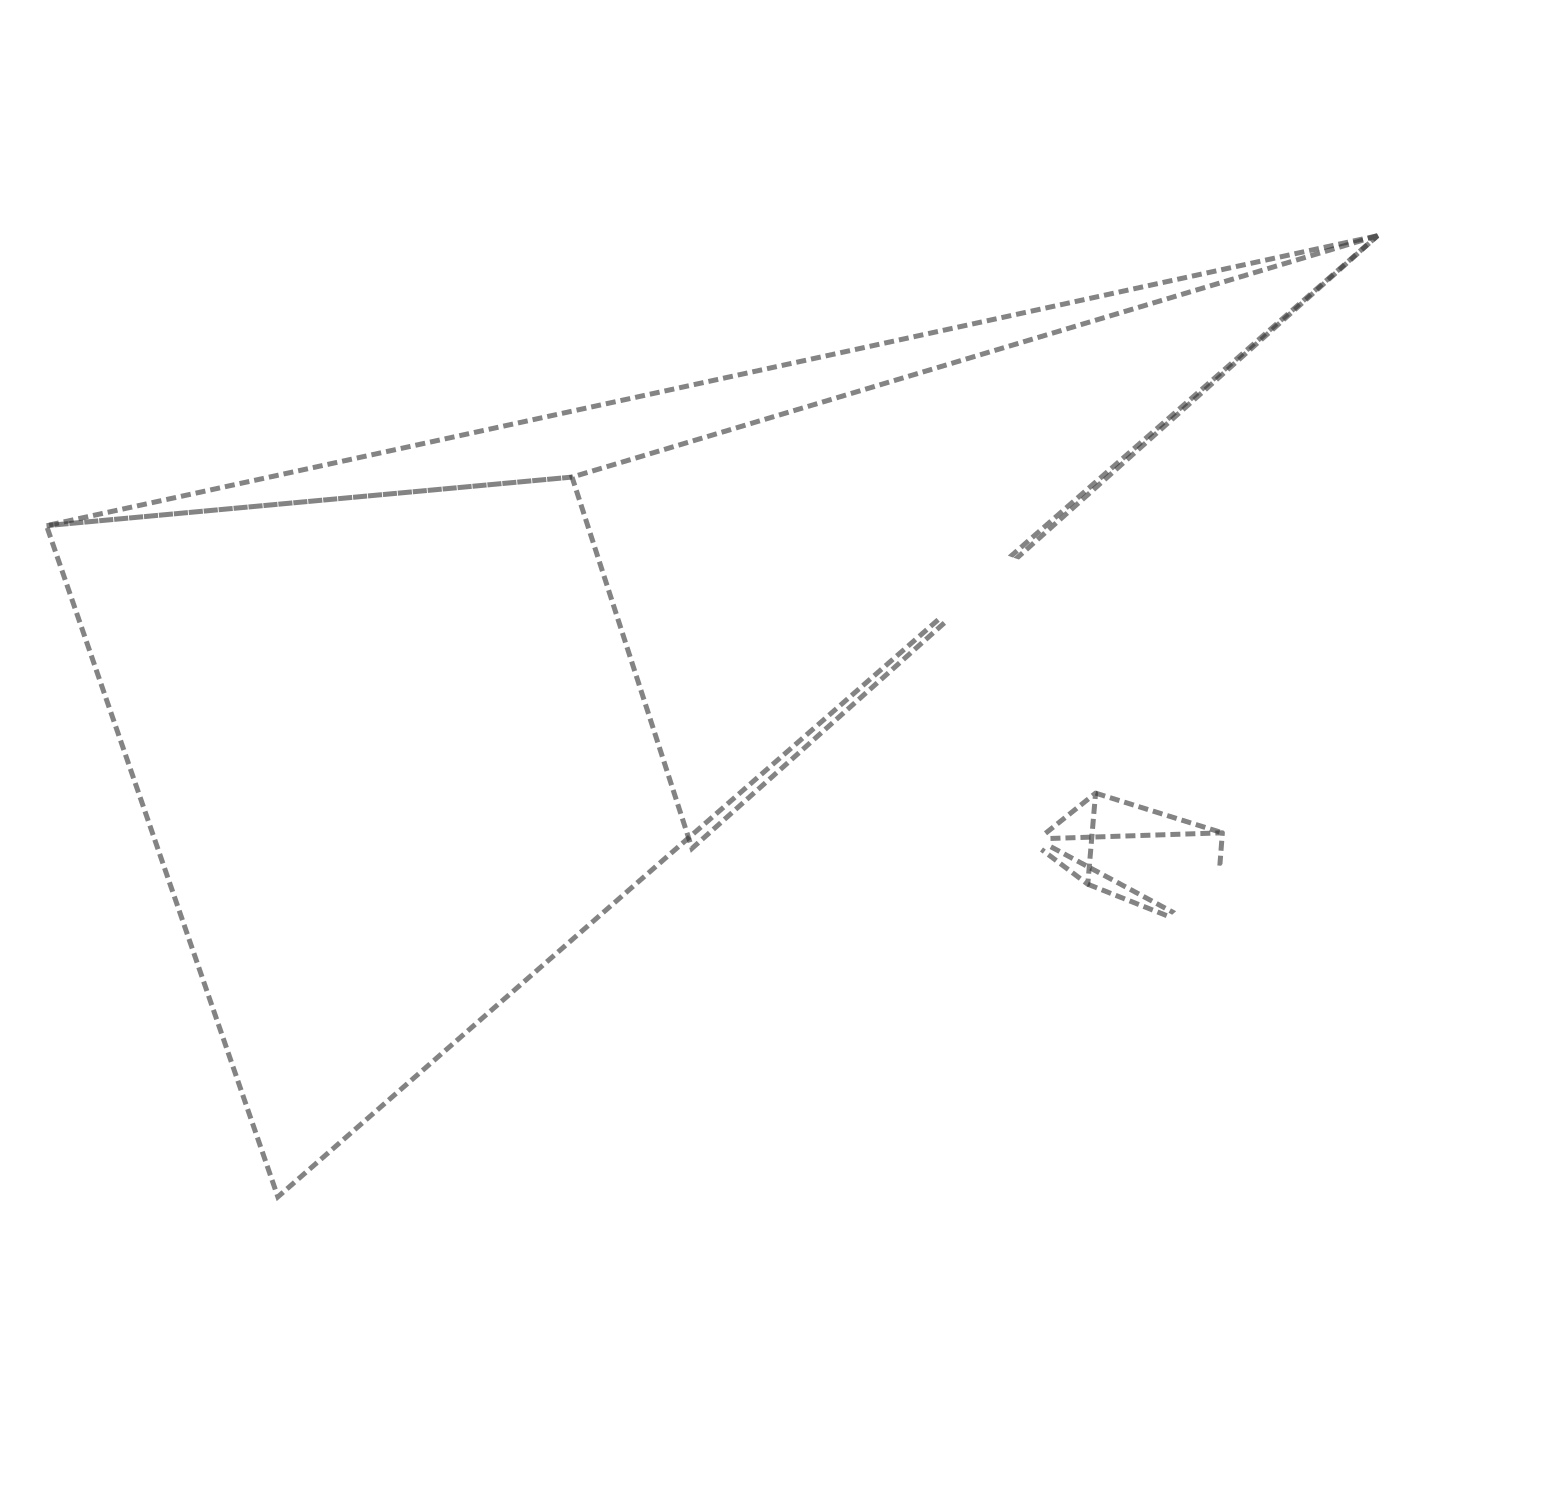
\includegraphics[width=\linewidth]{human-perspective-small}

                {\scriptsize
                \begin{itemize}
                    \item real-time situation assessment
                    \item geometric reasoning
                    \item perspective-taking
                \end{itemize}
                }

            \end{column}
            \begin{column}{0.4\linewidth}

                \begin{figure}

                    \resizebox{\columnwidth}{!}{%
                        \begin{tikzpicture}[
                                yscale=1.3,
                                >=latex,
                                every edge/.style={<-, draw, very thick},
                                every node/.style={draw, font=\sf, node distance=0.5, rounded corners,
                                align=center, inner sep=5pt,fill=hriSec2Dark!50},
                                classof/.style={<-, draw=black!60, dashed},
                                property/.style={<-, draw=hriSec2Comp},
                                propname/.style={above, draw=none, fill=none, font=\tt, inner sep=2pt},
                                instance/.style={draw=hriSec1Dark, font=\sf, node distance=0.5, rounded corners,
                                align=center, inner sep=5pt, fill=none}]

                            \node[fill=hriSec2Comp!50] (thing) {\textbf{thing}};
                            \node [fill=hriSec3CompDark!50, node distance=1.8, below left=of
                            thing](sthing) {place} edge[dashed] (thing);
                            \node [fill=hriSec3CompDark!50, below left=of sthing] (agent) {agent} edge (sthing);
                            \node [fill=hriSec3CompDark!50, below=of sthing] (artifact) {artifact} edge (sthing);
                            \node [fill=hriSec3CompDark!50, below right=of sthing] (location) {physical
                            support} edge (sthing);
                            \node [fill=hriSec3CompDark!50, below right=of artifact] (table) {table}
                            edge (location) edge (artifact);


                            \node [node distance=1, below right=of thing] (tthing) {temporal thing} edge (thing);
                            \node [below right=of tthing] (evt) {event} edge[dashed] (tthing);
                            \node [below right=of evt] (act) {action} edge (evt);

                            \uncover<2->{
                                \draw[dotted, thick] (-8,-3.8) -- +(16, 0);

                                \node [instance, below=3 of agent] (human) {human\_1} edge[classof, bend left] (agent);
                                \node [instance, above left=of human] (human2) {human\_2} edge[classof, bend left] (agent);
                                \node [instance, above right=of human, anchor=south] (robot) {myself} edge[classof, bend left] (agent);
                                \node [instance, right=of human, anchor=north west] (book) {book\_game\_thrones}
                                edge[classof] (artifact);
                                \node [instance, right=2 of robot] (ikea) {ikea\_table} edge[classof, bend
                                right] (table);
                                \node [instance, right=2 of book] (brown) {brown} edge[property] node[propname] {hasColor} (book);


                            }
                            \uncover<3->{
                                \draw[dotted, thick] (-8,-6.2) -- +(16, 0);

                                \node [instance, below=5 of act] (moving) {move\_act\_42} edge[classof] (act);
                                \path (moving.west) edge [property, out=180, in=-80, looseness=1] node[propname,below] {currentlyPerforms} (human.230);
                                \path (human.280) edge [property, out=-80, in=-90, looseness=3.5] node[propname,right] {looksAt} (robot.south);
                                \path (ikea.south) edge [property, out=-90, in=-80, looseness=2.5] node[propname, auto] {isOn} (book.320);
                            }
                        \end{tikzpicture}
                        }

                \end{figure}

                {\scriptsize
                \begin{itemize}
                    \item ontologies
                    \item real-time symbolic reasoning
                    \item theory of mind
                \end{itemize}
                }

            \end{column}
            \begin{column}{0.3\linewidth}
                \centering
                \resizebox{\columnwidth}{!}{%
                    \begin{tikzpicture}[
                            >=latex,
                            every edge/.style={draw, ultra thick, ->},
                            every node/.style={align=center},
                            robot/.style={fill=hriSec2Comp!50},
                            plan/.style={draw,
                            thick,  
                            circle, 
                            font=\sf,
                            align=center,
                            fill=hriSec3CompDark!50, 
                            minimum size=1cm, 
                            inner sep=0.1cm}
                        ]

                        \coordinate (figbottom) at (-0.5, -28.5);


                        \fill[gray!10!white] (4.6,.5) rectangle (figbottom);

                        \path (-0.5,0) edge (figbottom) node[sloped, above left, rotate=90] {\large\bf time};

                        \node at (2,0) (percept) {\bf Perception};
                        \node[below=0.5 of percept.south west, anchor=mid] {camera};
                        \node[below=0.5 of percept.south east, anchor=mid] {3D model};

                        \node[right=4 of percept, minimum width=2.5cm] (kb) {\bf Knowledge};
                        \node[below=0.5 of kb.south west, anchor=mid east] (kbr) {robot};
                        \node[below=0.5 of kb.south east, anchor=mid west] (kbh) {human};
                        \draw[dotted] (kbr) to (figbottom -| kbr);
                        \draw[dotted] (kbh) to (figbottom -| kbh);

                        \fill[gray!10!white] (12,.5) rectangle (17,0 |- figbottom);
                        \node[right=4.5 of kb] (plan) {\bf Plan};
                        \node[below=0.5 of plan.south west, anchor=mid east] (probot) {robot};
                        \node[below=0.5 of plan.south east, anchor=mid west] (phuman) {human};
                        \draw[dotted] (probot) to (figbottom -| probot);
                        \draw[dotted] (phuman) to (figbottom -| phuman);

                        \node[right=5 of plan] (action) {\bf Actions};
                        \node[below=0.5 of action.south west, anchor=mid east] (arobot) {robot};
                        \node[below=0.5 of action.south east, anchor=west] (ahuman) {human\\(monitoring)};
                        \draw[dotted] (arobot) to (figbottom -| arobot);
                        \draw[dotted] (ahuman) to (figbottom -| ahuman);

                        \draw[dashed] (-0.6,-1.2) --(24, -1.2);

                        \node[anchor=east] at (-0.5, -3) (t1) {\Large $t_1$};
                        \node[anchor=east, below=6 of t1] (t2) {\Large $t_2$};
                        \node[anchor=east, below=6 of t2] (t3) {\Large $t_3$};
                        \node[anchor=east, below=4 of t3] (t4) {\Large $t_4$};
                        \node[anchor=east, below=5 of t4] (t5) {\Large $t_5$};

                        %%%%%%%%%%%%%%%%%%%%%%%%%%%%%%%%%%%%%%%%%%%%%%%%%%%%%%%%%%%%%%%%%%%%%%%%%%%%%%%%%%%%%%%%%%%%
                        %%% PERCEPTIONS
                        %%%%%%%%%%%%%%%%%%%%%%%%%%%%%%%%%%%%%%%%%%%%%%%%%%%%%%%%%%%%%%%%%%%%%%%%%%%%%%%%%%%%%%%%%%%%

                        \node at (t1 -| percept) (cam1) {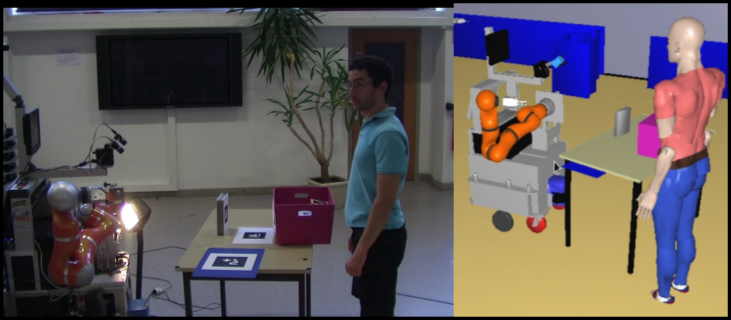
\includegraphics[height=2cm]{cleantable/manip_run_cam1.png}};
                        \node at (t2 -| percept) (cam2) {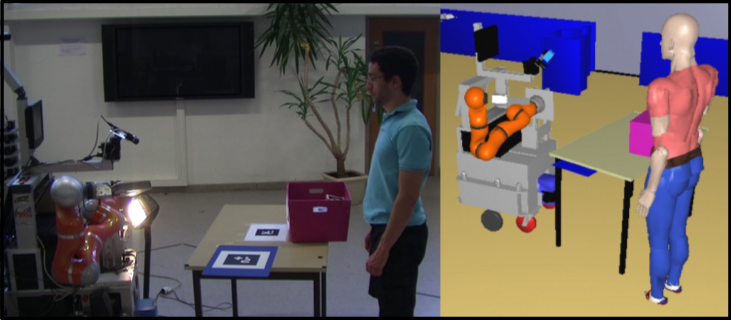
\includegraphics[height=2cm]{cleantable/manip_run_cam2.png}};
                        \node at (t3 -| percept) (cam3) {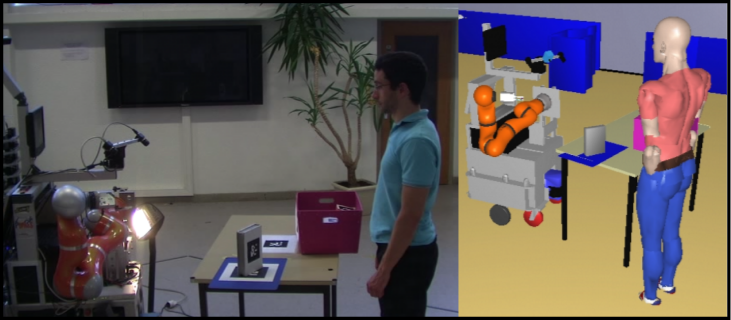
\includegraphics[height=2cm]{cleantable/manip_run_cam3.png}};
                        \node at (t4 -| percept) (cam4) {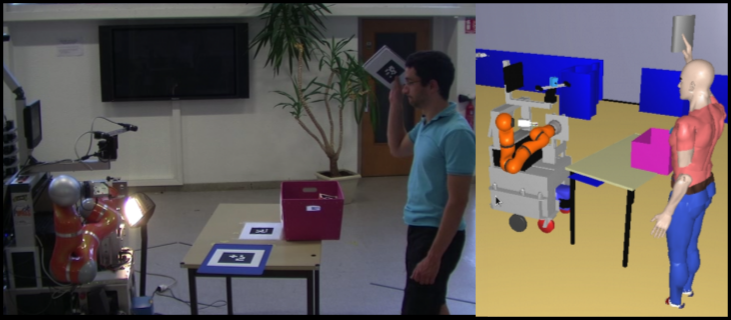
\includegraphics[height=2cm]{cleantable/manip_run_cam4.png}};
                        \node at (t5 -| percept) (cam5) {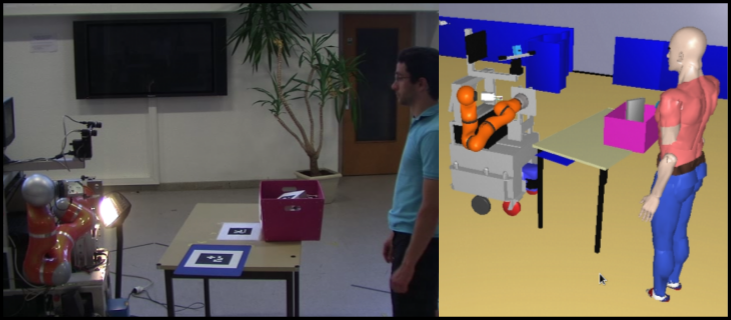
\includegraphics[height=2cm]{cleantable/manip_run_cam5.png}};

                        %%%%%%%%%%%%%%%%%%%%%%%%%%%%%%%%%%%%%%%%%%%%%%%%%%%%%%%%%%%%%%%%%%%%%%%%%%%%%%%%%%%%%%%%%%%%
                        %%% KNOWLEDGE
                        %%%%%%%%%%%%%%%%%%%%%%%%%%%%%%%%%%%%%%%%%%%%%%%%%%%%%%%%%%%%%%%%%%%%%%%%%%%%%%%%%%%%%%%%%%%%

                        \node[fill=white,align=left] at (cam1 -| kbr) (kb1) {\stmt{TAPE isVisible true}\\
                        \stmt{TAPE isReachable true}\\
                        \stmt{TAPE isOn TABLE}\\
                        \stmt{BIN isVisible true}\\
                        \stmt{BIN isReachable false}};

                        \node[fill=white,align=left] at (cam1 -| kbh) {\stmt{TAPE isVisible true}\\
                        \stmt{TAPE isReachable false}\\
                        \stmt{TAPE isOn TABLE}\\
                        \stmt{BIN isVisible true}\\
                        \stmt{BIN isReachable true}};

                        \node[fill=white,align=left] at (cam2 -| kbr) (kb2) {\stmt{ROBOT hasInHand TAPE}};


                        \node[fill=white,align=left] at (cam3 -| kbr) {\stmt{TAPE isReachable true}\\
                        \stmt{TAPE isVisible true} \\
                        \stmt{TAPE isOn TABLE}};

                        \node[fill=white,align=left ] at (cam3 -| kbh) (kb3) {\stmt{TAPE isReachable true}\\
                        \stmt{TAPE isVisible true}};

                        \node[fill=white,align=left] at (cam4 -| kbh) (kb4) {\stmt{HUMAN hasInHand TAPE}};

                        \node[fill=white,align=left] at (cam5 -| kbr)  {\stmt{TAPE isIn BIN}};
                        \node[fill=white,align=left] at (cam5 -| kbh) (kb5) {\stmt{TAPE isIn BIN}};

                        %%%%%%%%%%%%%%%% %%%%%%%%%%%%%%%%%%%%%%%%%%%%%%%%%%%%%%%%%%%%%%%%%%%%%%%%%%%%%%%%%%%%%%%%%%%%
                        %%% PLANS
                        %%%%%%%%%%%%%%%%%%%%%%%%%%%%%%%%%%%%%%%%%%%%%%%%%%%%%%%%%%%%%%%%%%%%%%%%%%%%%%%%%%%%%%%%%%%%

                        \node[fill=gray!10!white,below=1 of plan] (incoming) {\bf \Large Incoming goal \\ \it Clean the table!};

                        \node[anchor=north, plan, robot] at (cam1.south -| probot) (pr1) {\bf TAKE\\TAPE\\TABLE};
                        \node[anchor=north, plan, robot] at (cam2.south -| probot)  (pr2) {\bf PUTRV\\TAPE\\TABLE} edge[<-] (pr1);
                        \node[anchor=north, plan] at (cam3.south -| phuman) (ph1) {\bf TAKE\\TAPE\\TABLE} edge[<-] (pr2);
                        \node[anchor=north, plan]  at (cam4.south -| phuman) (ph2) {\bf PUT\\TAPE\\BIN} edge[<-] (ph1);

                        \node[fill=gray!10!white,anchor=north] at (cam5.south -| plan) (done) {\bf \Large Goal completed};

                        %%%%%%%%%%%%%%%%%%%%%%%%%%%%%%%%%%%%%%%%%%%%%%%%%%%%%%%%%%%%%%%%%%%%%%%%%%%%%%%%%%%%%%%%%%%%
                        %%% ACTIONS
                        %%%%%%%%%%%%%%%%%%%%%%%%%%%%%%%%%%%%%%%%%%%%%%%%%%%%%%%%%%%%%%%%%%%%%%%%%%%%%%%%%%%%%%%%%%%%

                        \only{
                            \node[fill=white] at (pr1 -| arobot) (ep1) {\it evaluate pre-conditions};

                            \node[below=0.1 of ep1] (mhp1) {%
                                \begin{tikzpicture}
                                    \node[fill=white] (title) {\bf motion planning};
                                    \node[below=0.1 of title.south west, label=below:{\tt PICK\_GOTO}] (mapg) {
\includegraphics{cleantable/MHP_ARM_PICK_GOTO}};
                                    \node[fill=white,right=of mapg, label=below:{\tt TAKE\_TO\_FREE}] (mattf) {
\includegraphics{cleantable/MHP_ARM_TAKE_TO_FREE}} edge[<-] (mapg);
                                \end{tikzpicture}
                                };
                                \node[fill=white,below=0.1 of mhp1] (me1) {\bf motion execution};
                                \node[fill=white,below=0.1 of me1] (ae1) {\it assess post-conditions};
                            }
                            %%%%%%%%%%%%%%%%%%%%%%%%%%%%%%%%%%%%%%%%%%%%%%%%%%%%%%%%%%%%%%%%%%%%%%%%%%%%%%%%%%%%%%%%%%%%%
                            \only{
                                \node[fill=white] at (pr2 -| arobot) (ep2) {\it evaluate pre-conditions};

                                \node[below=0.1 of ep2] (mhp2) {%
                                    \begin{tikzpicture}
                                        \node[fill=white] (title) {\bf motion planning};
                                        \node[fill=white,below=0.1 of title, label=below:{\tt ESCAPE}] (maeo) {
\includegraphics{cleantable/MHP_ARM_ESCAPE_OBJECT}};
                                        \node[left=of maeo, label=below:{\tt PLACE\_FROM\_FREE}] (mapff) {
\includegraphics{cleantable/MHP_ARM_PLACE_FROM_FREE}} edge (maeo);
                                        \node[fill=white,right=of maeo, label=below:{\tt TO\_FREE}] (maf) {
\includegraphics{cleantable/MHP_ARM_FREE}} edge[<-] (maeo);
                                    \end{tikzpicture}
                                    };
                                    \node[fill=white,below=0.1 of mhp2] (me2) {\bf motion execution};
                                    \node[fill=white,below=0.1 of me2] (ae2) {\it assess post-conditions};
                                }
                                %%%%%%%%%%%%%%%%%%%%%%%%%%%%%%%%%%%%%%%%%%%%%%%%%%%%%%%%%%%%%%%%%%%%%%%%%%%%%%%%%%%%%%%%%%%%%

                                \node[anchor=north] at (ph1 -| ahuman) (wait1) {%
                                    \begin{tikzpicture}
                                        \node[fill=white] (title) {\it wait for pick\\ {\tt TAPE} \it from {\tt TABLE}};
                                        \node[below=0.1 of title] {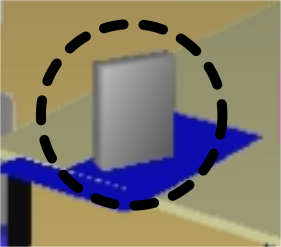
\includegraphics{cleantable/wait_for_pick}};
                                    \end{tikzpicture}
                                    };

                                    \node[anchor=north] at (ph2 -| ahuman) (wait2) {%
                                        \begin{tikzpicture}
                                            \node[fill=white] (title) {\it wait for put\\ {\tt TAPE} \it into {\tt BIN}};
                                            \node[below=0.1 of title] {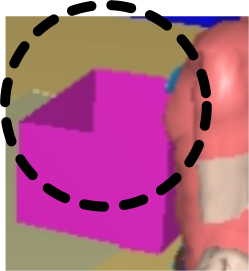
\includegraphics{cleantable/wait_for_throw}};
                                        \end{tikzpicture}
                                        };


                                        %%%%%%%%%%%%%%%%%%%%%%%%%%%%%%%%%%%%%%%%%%%%%%%%%%%%%%%%%%%%%%%%%%%%%%%%%%%%%%%%%%%%%%%%%%%%
                                        %%% FLOW
                                        %%%%%%%%%%%%%%%%%%%%%%%%%%%%%%%%%%%%%%%%%%%%%%%%%%%%%%%%%%%%%%%%%%%%%%%%%%%%%%%%%%%%%%%%%%%%
                                        \draw[dotted, ->, in=45, out=180] (incoming.west) to (kb1);
                                        \draw[dotted, ->, bend right] (kb1) to (pr1);
                                        \draw[dotted, ->, bend left] (pr1) to (ep1);
                                        \draw[dotted, ->, in=45, out=180] (ae1.west) to (kb2);
                                        \draw[dotted, ->, bend right] (kb2) to (pr2);
                                        \draw[dotted, ->, bend left] (pr2) to (ep2);
                                        \draw[dotted, ->, in=45, out=180] (ae2.west) to (kb3);
                                        \draw[dotted, ->, bend right] (kb3) to (ph1);
                                        \draw[dotted, ->, bend left] (ph1) to (wait1);
                                        \draw[dotted, ->, in=-20, out=180] (wait1.west) to (kb4.east);
                                        \draw[dotted, ->, bend right] (kb4) to (ph2);
                                        \draw[dotted, ->, bend left] (ph2) to (wait2);
                                        \draw[dotted, ->, in=20, out=180] (wait2.west) to (kb5);
                                        \draw[dotted, ->, bend left] (kb5.east) to (done.north);


                        \end{tikzpicture}
                        }

                    {\scriptsize
                    \begin{itemize}
                        \item Complete cognitive architecture
                        \item Autonomy in semantic-rich social environments
                    \end{itemize}
                    }
                    \end{column}
                \end{columns}

            \end{frame}
            }

{
    \paper{Mohamed, Lemaignan \textbf{ROS for Human-Robot Interaction} Arxiv
    2021 (under review IROS)}

\begin{frame}{REAL-WORLD SOCIAL AUTONOMY --- social signal processing}
    \begin{center}
        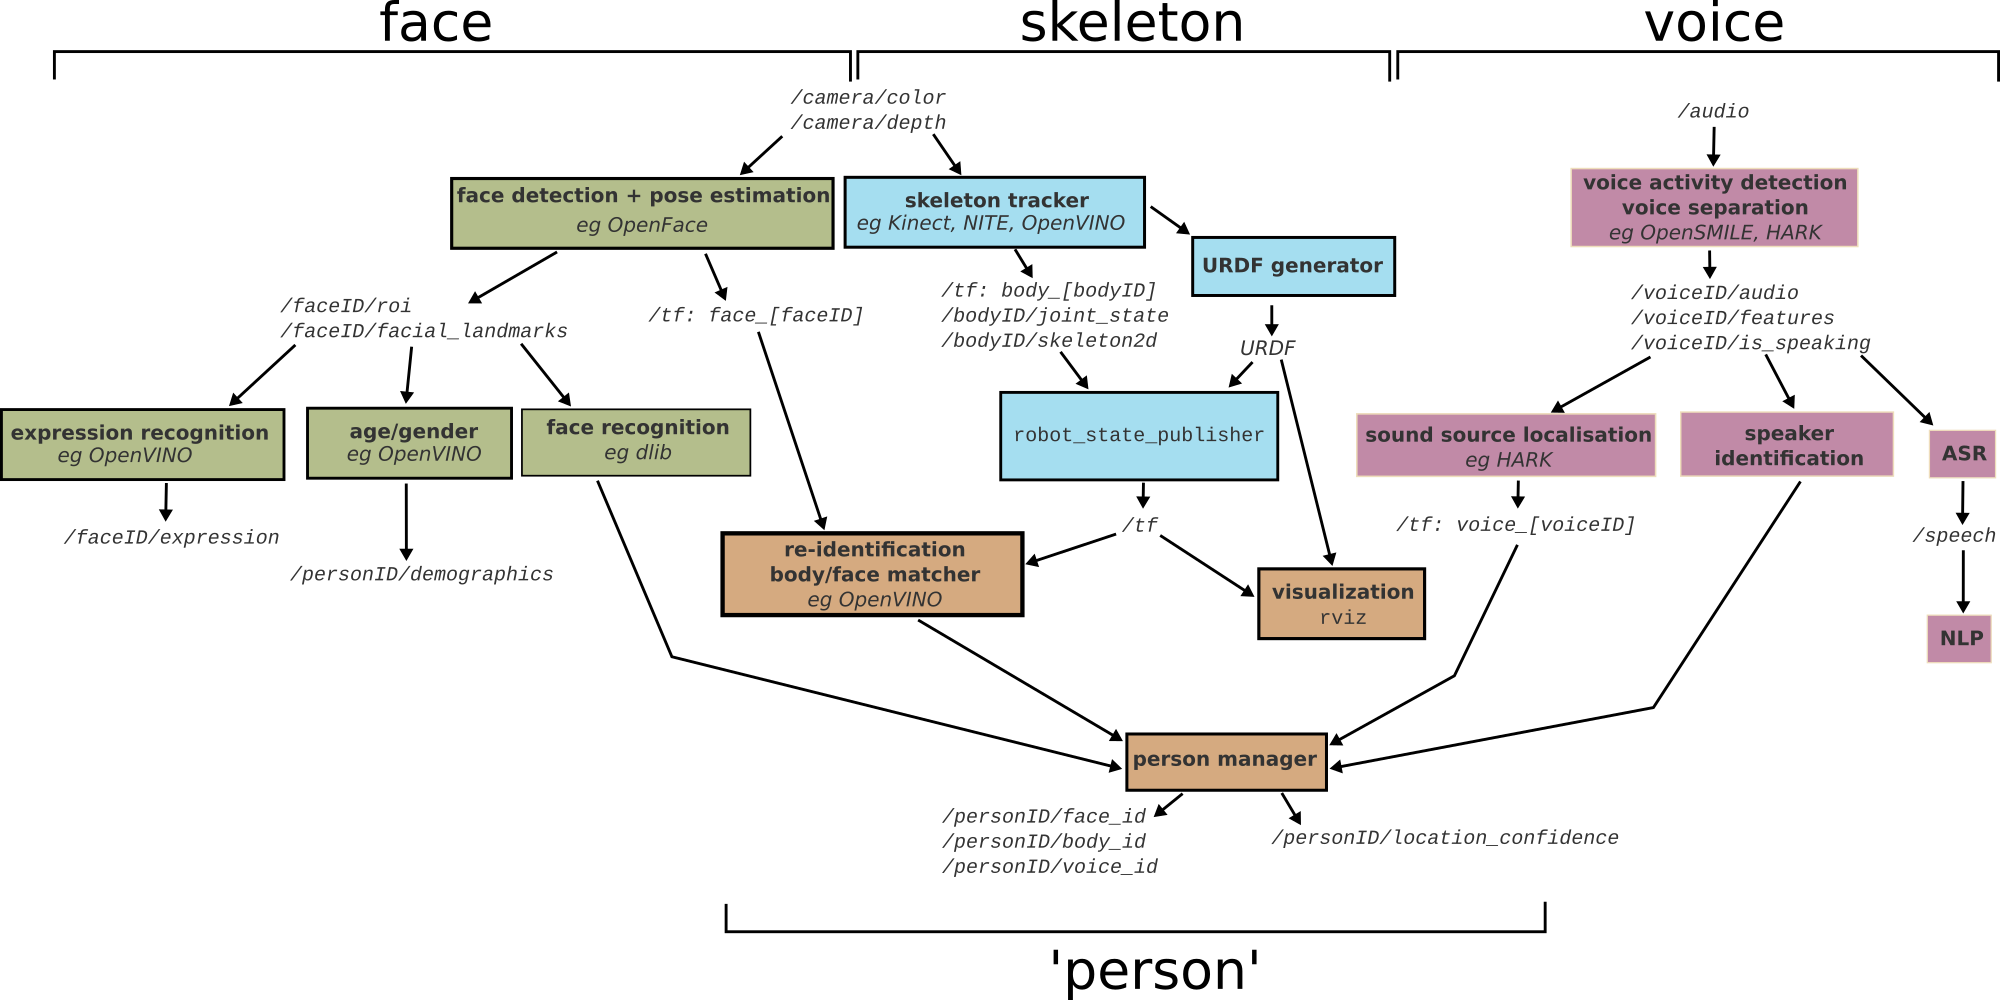
\includegraphics[width=\columnwidth]{architectures/ros4hri-pipeline}
    \end{center}
    ROS4HRI: first integrated, multi-modal, ROS-based pipeline for social signal
    processing in robotics
\end{frame}
}


%%%%%%%%%%%%%%%%%%%%%%%%%%%%%%%%%%%%%%%%%%%%%%%%%%%%%%%%%%%%%%%%%%%%%%%%%%%%%%%%%%%%%%%%%
%%%%%%%%%%%%%%%%%%%%%%%%%%%%%%%%%%%%%%%%%%%%%%%%%%%%%%%%%%%%%%%%%%%%%%%%%%%%%%%%%%%%%%%%%

%\imageframe[color=black]{social-interactions/social-interactions.pdf}

{
    \paper{Lemaignan et al. \textbf{The PInSoRo dataset: Supporting the data-driven study of child-child and child-robot [...]} PLOS One 2018]

    [Bartlett et al. \textbf{What Can You See? Identifying Cues on Internal States from the Kinematics [...]} FrontiersIn 2019}

\begin{frame}{DATA-DRIVEN HRI --- dataset of natural interactions}
    \begin{columns}
        \begin{column}{0.5\linewidth}
            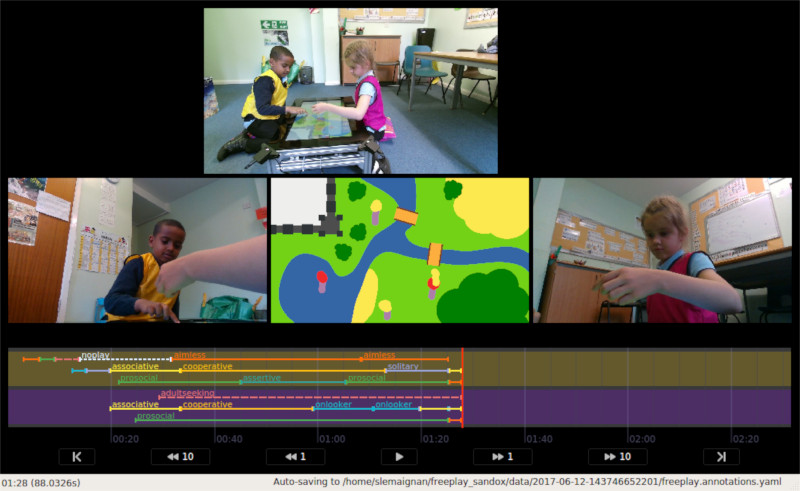
\includegraphics[width=\columnwidth]{pinsoro/annotator.jpg}
        \end{column}
        \begin{column}{0.5\linewidth}
            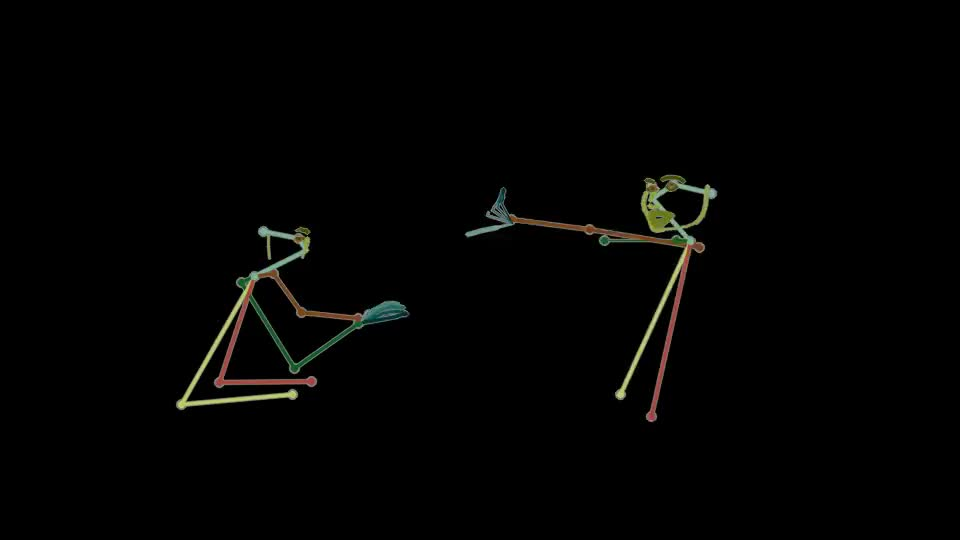
\includegraphics[width=\columnwidth]{kinematics_social_dynamics/clip_skel_05_thumb.jpg}

        \end{column}
    \end{columns}
    \vspace{0.5cm}
\begin{columns}
    \begin{column}{0.5\linewidth}
        {\scriptsize
        \begin{itemize}
            \item PInSoRo dataset: 45h+ and 2M frames of annotated natural interactions
            \item new data analysis techniques to estimate internal state from body language
            \item first-in-kind dataset for data-driven study of social
                interactions in robotics
        \end{itemize}
        }
    \end{column}
    \begin{column}{0.5\linewidth}
            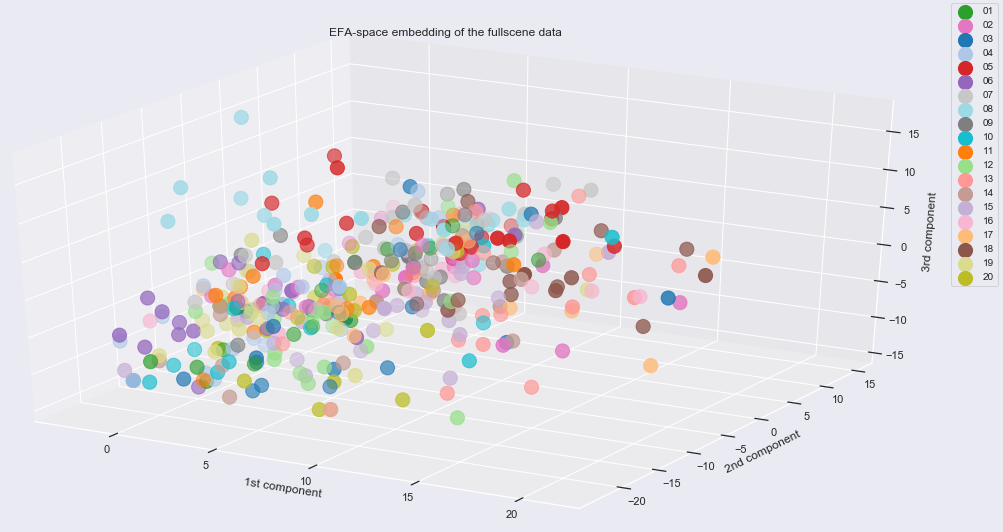
\includegraphics[trim=1cm 0 4cm 0,clip,width=\columnwidth]{kinematics_social_dynamics/efa-embeddings.png}
    \end{column}
\end{columns}

\end{frame}
}

{
    \paper{Senft et al. \textbf{Teaching robots social autonomy from in situ
    human guidance} Science Robotics 2019]

    [Winkle et al. \textbf{In-Situ Learning from a Domain Expert for Real World Socially Assistive Robot Deployment} RSS 2020}

\begin{frame}{DATA-DRIVEN HRI --- expert-in-the-loop machine learning}

    \begin{columns}
        \begin{column}{0.5\linewidth}
                \centering
                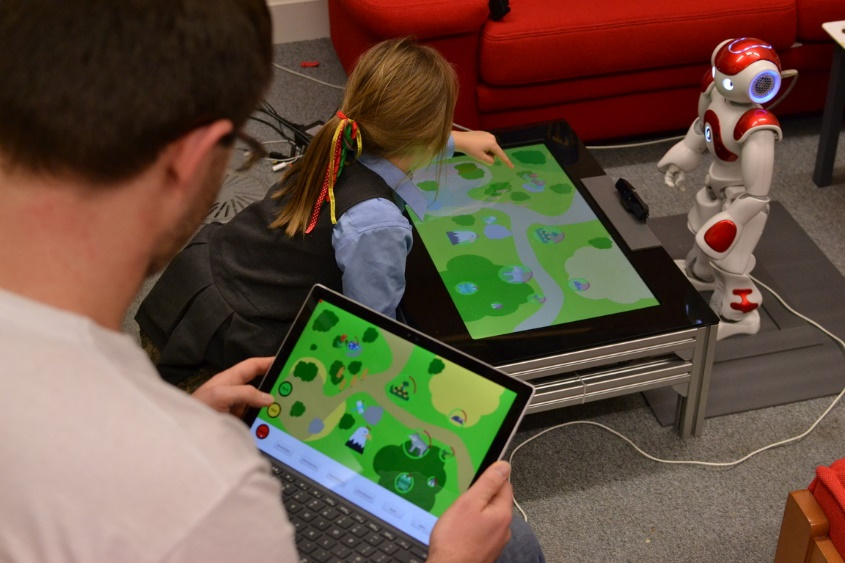
\includegraphics[height=3cm]{sparc/overview.jpg}
        \end{column}
        \begin{column}{0.5\linewidth}
                \centering
                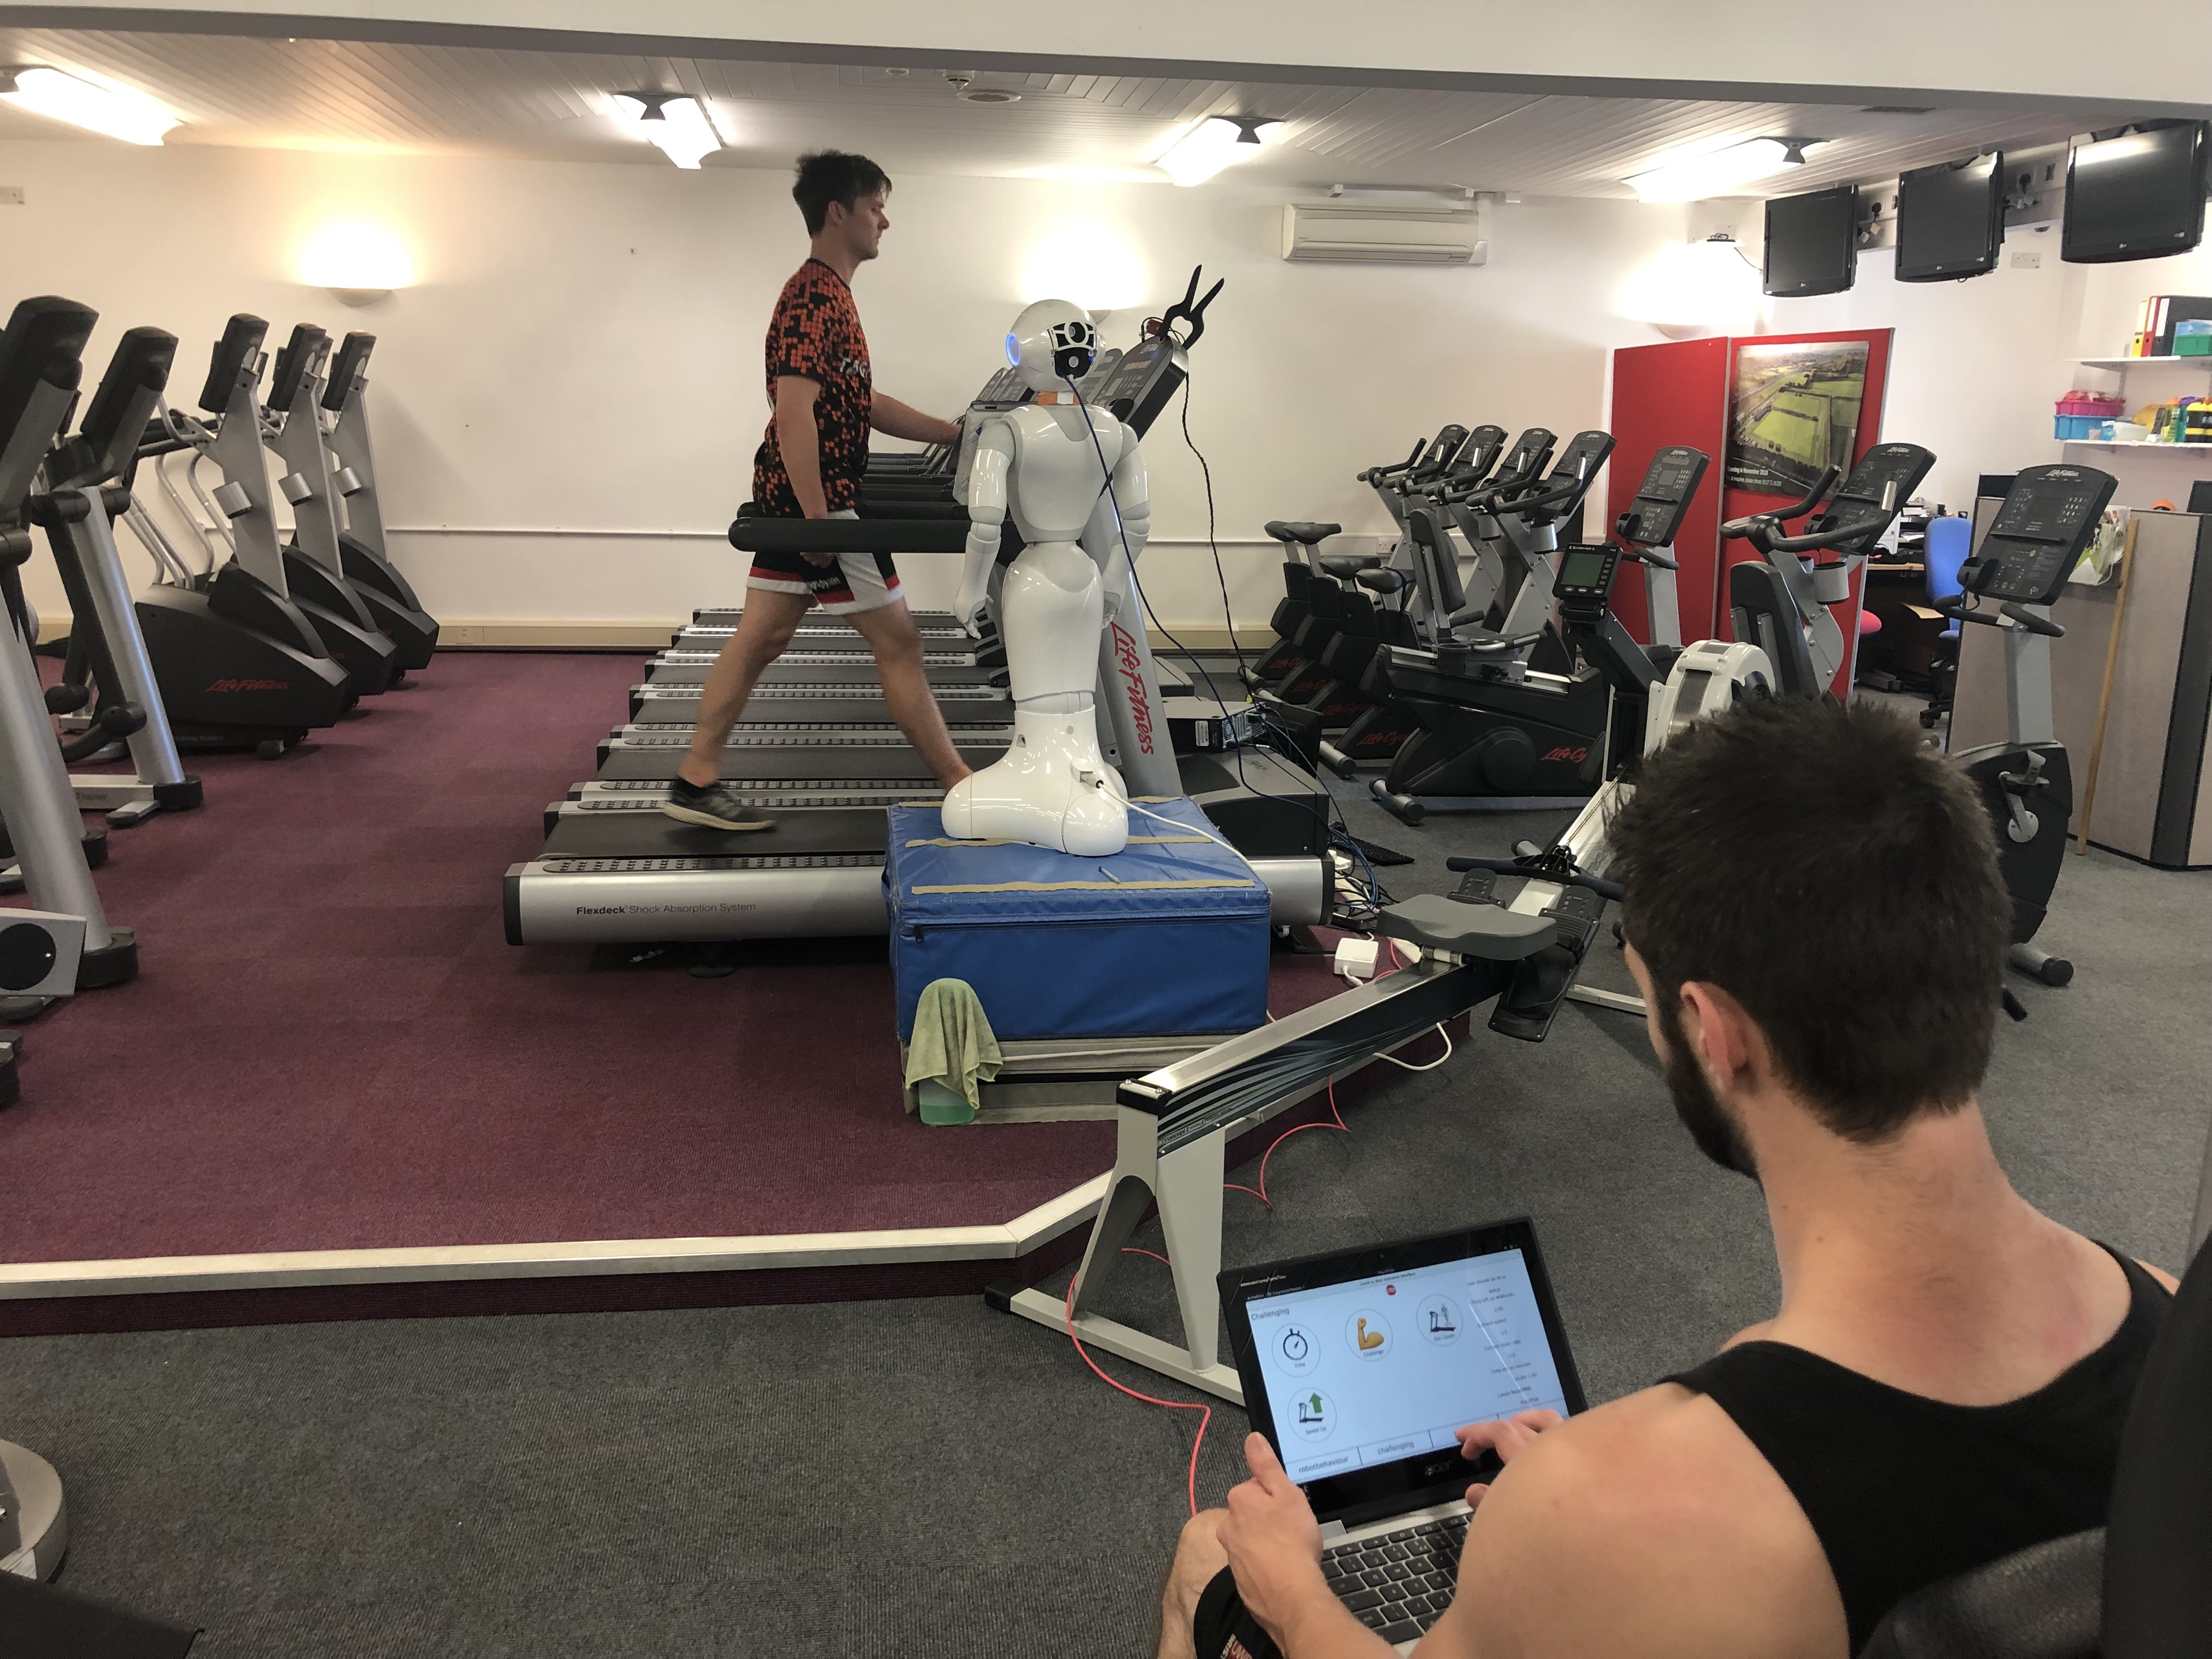
\includegraphics[height=3cm]{couch25k/supervised.jpg}
        \end{column}
    \end{columns}
        \centering
        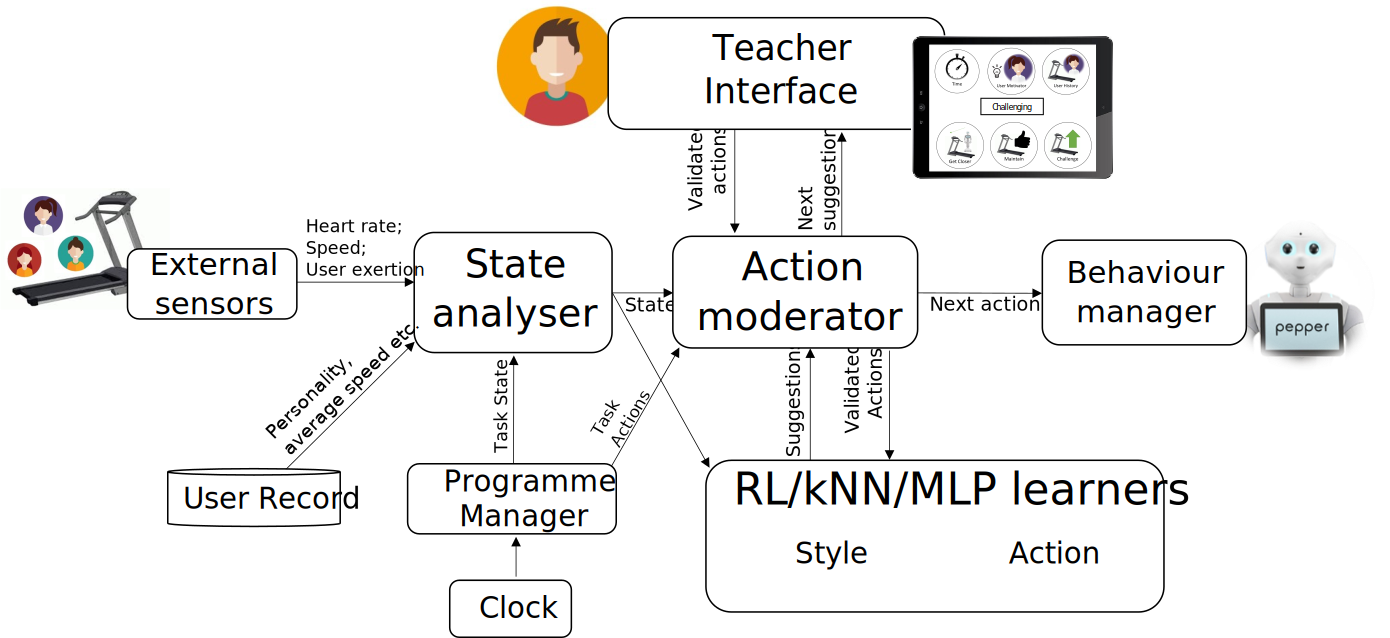
\includegraphics[height=4cm]{couch25k/architecture.pdf}
\end{frame}
}

%%%%%%%%%%%%%%%%%%%%%%%%%%%%%%%%%%%%%%%%%%%%%%%%%%%%%%%%


{
    \fullbackground{experiments-col}
\begin{frame}{HUMAN FACTORS --- experimental work}

    \begin{columns}
        \begin{column}{0.4\linewidth}

    Extensive experimental work:

    \begin{itemize}
        \item over 25 field experiments over the past 10 years
        \item focus on real-world experiments (eg schools, gyms) 
        \item child-robot interaction expertise: worked with 200+ children
    \end{itemize}

    \end{column}
        \begin{column}{0.6\linewidth}
    \end{column}
    \end{columns}
\end{frame}
}


\begin{frame}{HUMAN FACTORS --- expertise}

        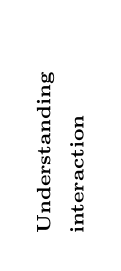
\begin{tikzpicture}
            \node[rotate=90,text width=2.5cm]{\scriptsize\textbf{Understanding\\interaction}};
        \end{tikzpicture}
            \hyperlink{croquignole}{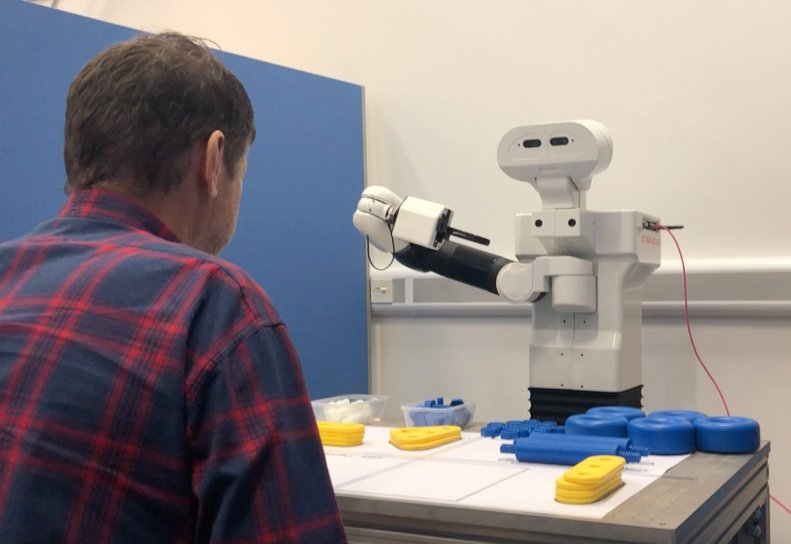
\includegraphics[height=0.2\paperheight]{trust/Tiago_and_participant}}
            \hspace{0.5em}
            \hyperlink{dominos}{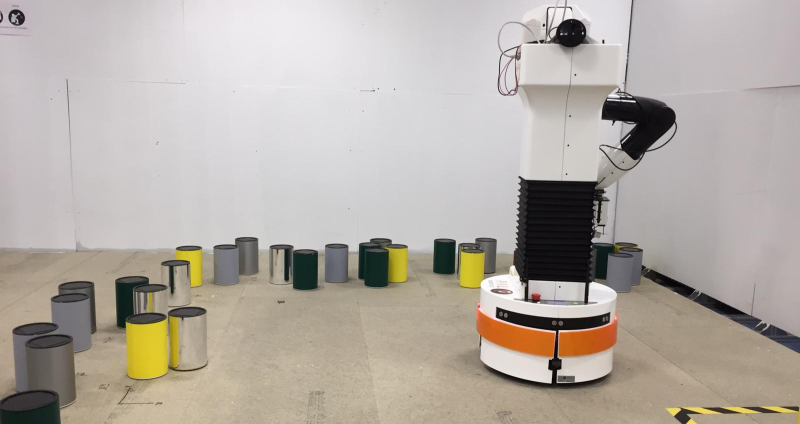
\includegraphics[trim=10cm 0 4cm 0,clip,height=0.2\paperheight]{dynamic-language/Preview_image}}
            \hspace{0.5em}
            \hyperlink{anthropomorphism}{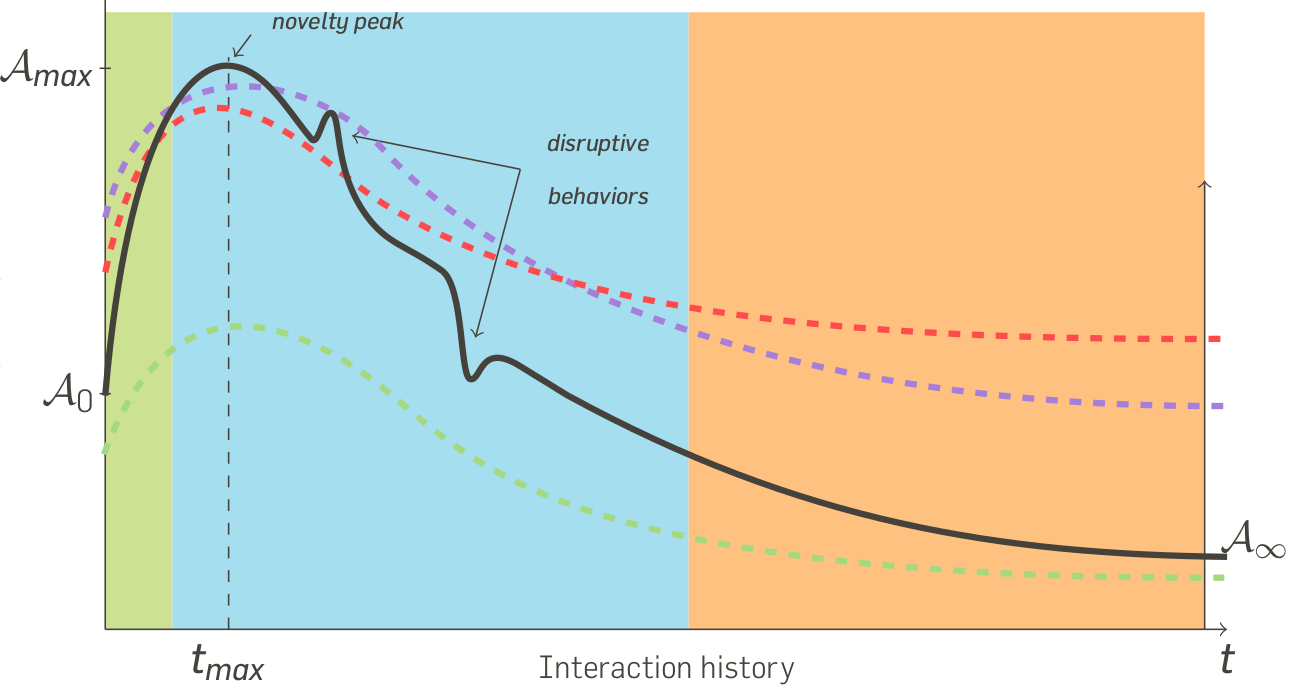
\includegraphics[height=0.2\paperheight]{dynamics_anthropo}}

        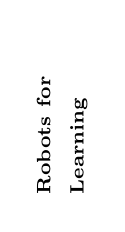
\begin{tikzpicture}
            \node[rotate=90,text width=2cm]{\scriptsize\textbf{Robots for \\Learning}};
        \end{tikzpicture}
            \hyperlink{cowriter}{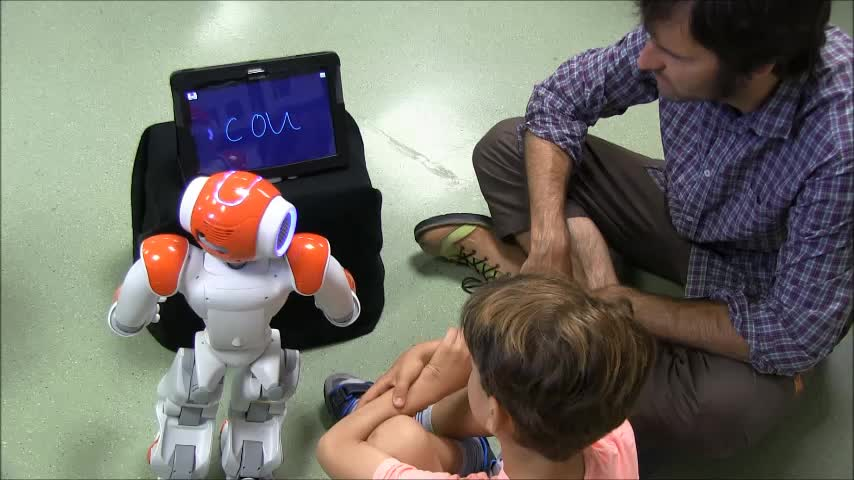
\includegraphics[height=0.2\paperheight]{cowriter/cowriter-session1_3minExcerpt_1x_thumb}}
            \hspace{0.5em}
            \hyperlink{cowriter-impl}{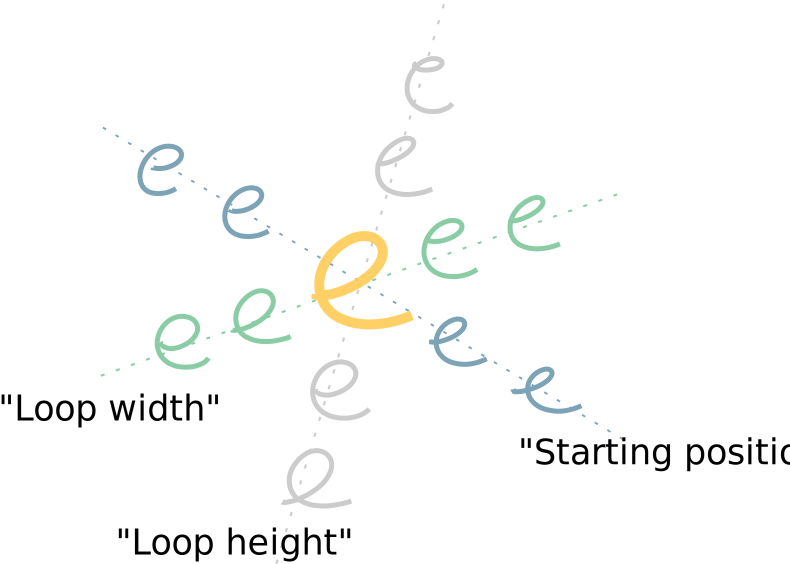
\includegraphics[height=0.2\paperheight]{cowriter/pca}}
            \hspace{0.5em}
            \hyperlink{cellulo}{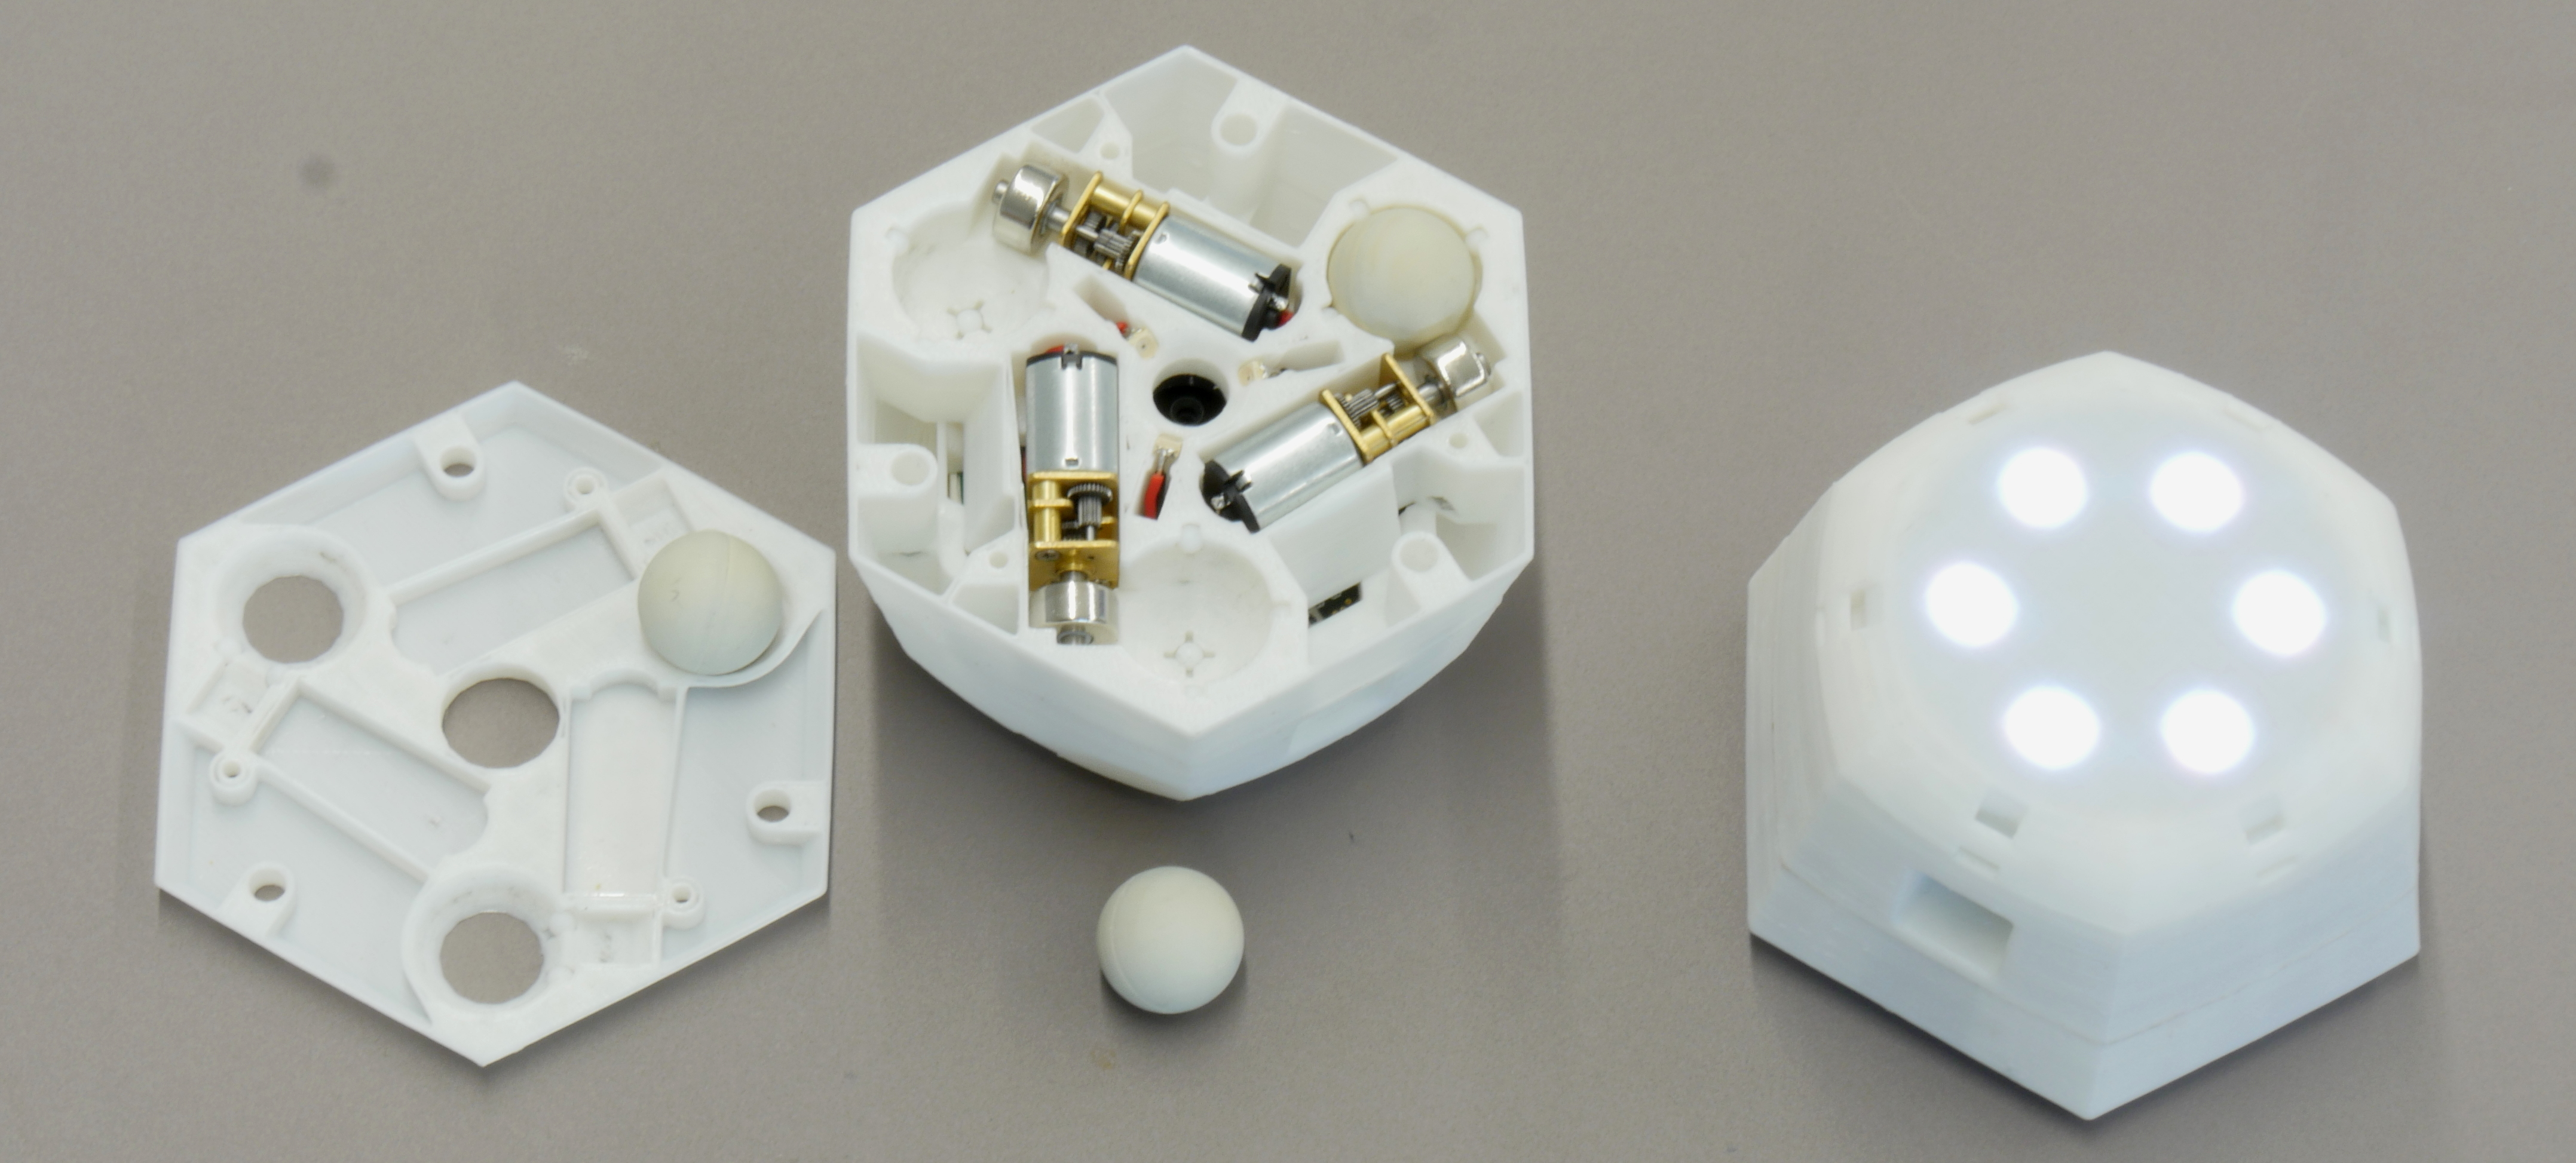
\includegraphics[trim=19cm 0 2cm 0,clip,height=0.2\paperheight]{cellulo/hardware-design-2}}

        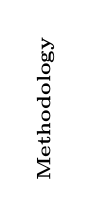
\begin{tikzpicture}
            \node[rotate=90]{\scriptsize\textbf{Methodology}};
        \end{tikzpicture}
            \hyperlink{withmeness}{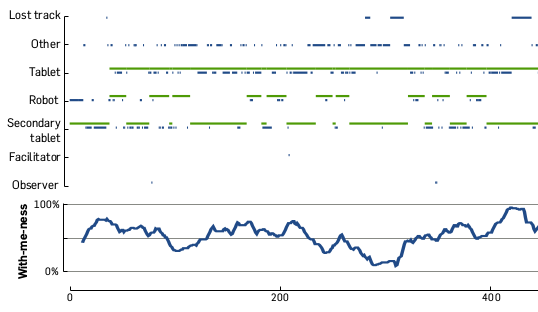
\includegraphics[height=0.2\paperheight]{withmeness/withmeness}}
            \hspace{0.5em}
            \hyperlink{asr}{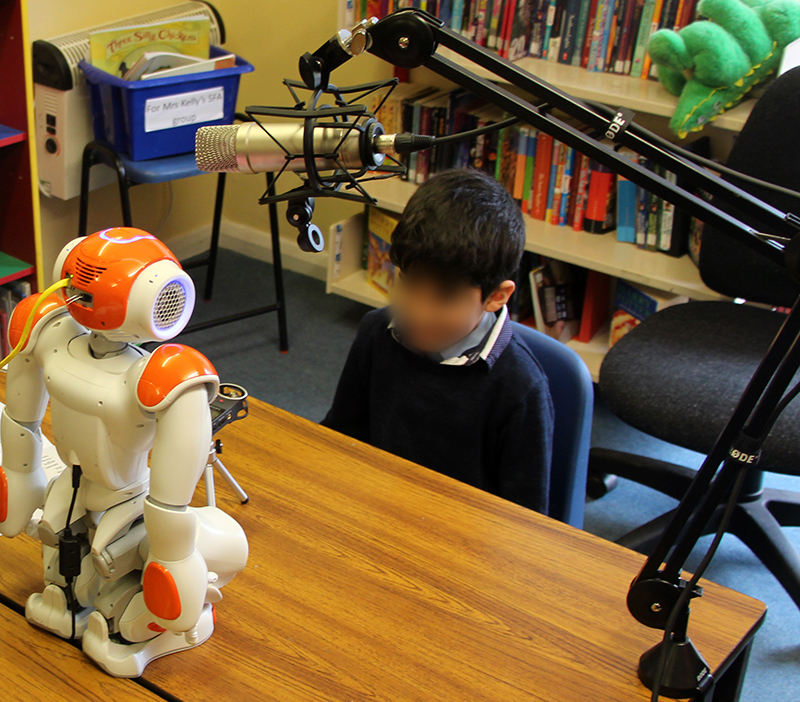
\includegraphics[height=0.2\paperheight]{speech-reco/record_img}}
            \hspace{0.5em}
            \hyperlink{constructs}{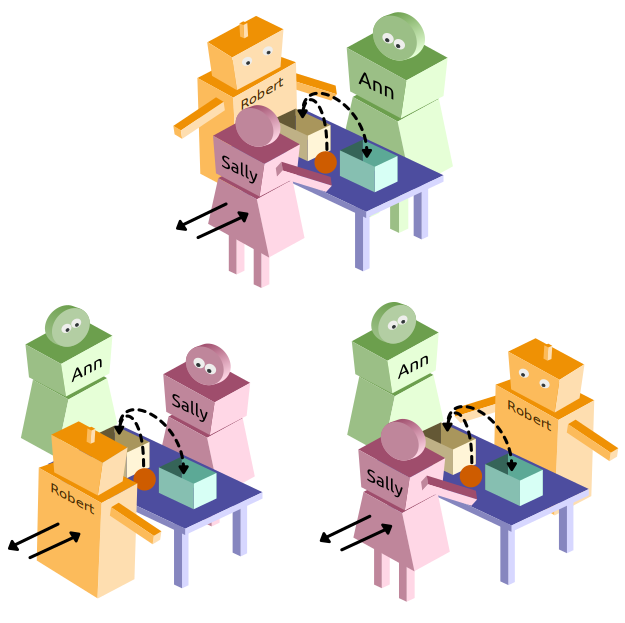
\includegraphics[height=0.2\paperheight]{triadic_false_beliefs}}
\end{frame}

\section*{Impact}

\begin{frame}{SCIENTIFIC IMPACT}

    Contributions to basic research, experimental methodology and technology:

    {\scriptsize
    \begin{enumerate}
        \item \textbf{ontologies} for robot knowledge modeling and symbolic
            reasoning
        \item \textbf{perspective taking} and \textbf{theory of mind}: generate and
            maintain symbolic knowledge models for all the agents
    %    \item large-scale, multi-modal, standard-compliant \textbf{social signal
    %        processing} for robots
        \item framing \& implementing \textbf{cognitive architecture for social interaction}
        \item leading role in \textbf{shaping the emergent field of data-driven
            HRI}: \textbf{large datasets}; transdisciplinary \textbf{data-driven behaviour analysis} 
        \item major advances towards \textbf{learning autonomous social policies} for service robots
        \item transdisciplinary expertise; number of \textbf{cross-disciplinary
            experimental work} and literature surveys;
        \item \textbf{Child-robot interaction} expert in Europe
    \end{enumerate}
    }

    {\scriptsize
    \begin{itemize}
        \item \textbf{75+ publications} (2800+ citations, h-index=26 on Google Scholar), incl. \emph{Artificial Intelligence},
            \emph{Science Robotics}
        \item Prix GdR Meilleure thèse
        \item Best Paper awards at RoMan, HRI
        \item major contributions to open-source robotics (core ROS dev); 150+ GitHub repos
    \end{itemize}
    }
\end{frame}


\begin{frame}{MANAGEMENT OF RESEARCH}
    \begin{itemize}
        \item \textbf{Associate professor in AI and Social Robotics}
        \item \textbf{Supervising 2 groups} at BRL (embodied cognition and autonomous
            vehicles), $\approx$\textbf{15 researchers}
        \item Responsible for \textbf{defining and implementing their research strategy}
        \item Currently managing \textbf{$>$€1M funding}
        \item Previously \textbf{established and led cHRI group at EPFL}; now
            internationally recognised
        \item Supervised or co-supervised \textbf{10 PhDs} to date
        \item \textbf{10+ years of teaching experience}; currently teaching HRI at Master
            level
    \end{itemize}

\end{frame}

\begin{frame}{IMPACT IN THE SCIENTIFIC COMMUNITY}

    Editorial activities

    \begin{itemize}
        \item Currently \textbf{Programme committee/editorial board} of FrontiersIn Robotics and
            AI; HRI; RSS; IROS; IJCAI
        \item \textbf{Organisation committee} of ACM/IEEE HRI since 2016
    \end{itemize}

    Bids and grants:
    \begin{itemize}
        \item PI or Co-I on \textbf{19 grant submissions} since 2013, incl. 4 EU ICT bids; 1
            EU FET bids; \textbf{5 successful to date}
        \item \textbf{EU H2020 Marie-Curie fellowship} on Theory of Mind in 2015
        \item First \textbf{ERC Consolidator submission} in 2019
    \end{itemize}


\end{frame}

\begin{frame}{IMPACT ON THE BROADER SOCIETY}

    Policy making:

    \begin{itemize}
        \item \textbf{EU Invited expert} on child-robot interaction
        \item \textbf{Scientific adivor for UNICEF} on ethics of cHRI
    \end{itemize}

    Technology transfer:
    \begin{itemize}
        \item \textbf{Scientific expert} for EU TERRINET, EU SABRE and 3 UK-based
            industry-led projects
        \item \textbf{Scientific advisor} for start-up KickSum Ltd
        \item US \textbf{patent} US20190016213A1 on haptic locomotion
    \end{itemize}

    Public engagement:
    \begin{itemize}
        \item Cluster \textbf{lead for outreach} at UWE
        \item Significant \textbf{media engagement} (TV, radio, press; eg CoWriter, Couck25K projects)
        \item Scientific engagement with public institutions, eg \textbf{London
            Science Museum}
    \end{itemize}

\end{frame}

\imageframe[scale=0.95]{collaborations_map}

%%%%%%%%%%%%%%%%%%%%%%%%%%%%%%%%%%%%%%%%%%%%%%%%%%%%%%%%%%%%%%%%%%%%%%%%%%%%%
%%%%%%%%%%%%%%%%%%%%%%%%%%%%%%%%%%%%%%%%%%%%%%%%%%%%%%%%%%%%%%%%%%%%%%%%%%%%%
\imageframe{my_background/00}

\miniframeson{}

\section{Research project}

\begin{frame}{SOCIAL ROBOTICS}
    \centering

    \begin{columns}
        \begin{column}{0.7\linewidth}

            \only<1>{
                Creating interactive robots that are \textbf{embedded and
                understand their (human) social context}; \textbf{generate and adopt appropriate
                social behaviours}; have a \textbf{positive impact on human
                society}.

                \vspace{2em}
                $\Rightarrow$ designing and implementing the \textbf{assistant and
                companion robots} for  tomorrow.

                \vspace{2em}
                $\Rightarrow$ direct impact on ageing society, education, customer service;
                \textbf{major societal
                challenge} \& \textbf{European priority}.
            }

            \only<2->{
                \textbf{Major scientific challenges}:

                \begin{itemize}
                    \item Understand and sustain long-term autonomous social interactions;
                    \item Real-world algorithmic robustness;
                    \item Complex ethical landscape;
                    \item $\Rightarrow$ cross-disciplinary \& holistic approach required
                \end{itemize}


                \uncover<3>{
                \vspace{2em}

                \textbf{My research proposal}:

                \setbeamercolor{hriSec1Demo}{bg=hriSec3Dark,fg=white}
                \begin{beamercolorbox}[wd=\linewidth,ht=8ex,dp=0.7ex]{hriSec1Demo}
                    \large \bf \centering
                    Socially-Driven Autonomous Robots \\
                    for \\
                    Real-world Human-Robot Interactions
                \end{beamercolorbox}
            }


            }
        \end{column}
        \begin{column}{0.3\linewidth}
            \begin{center}
                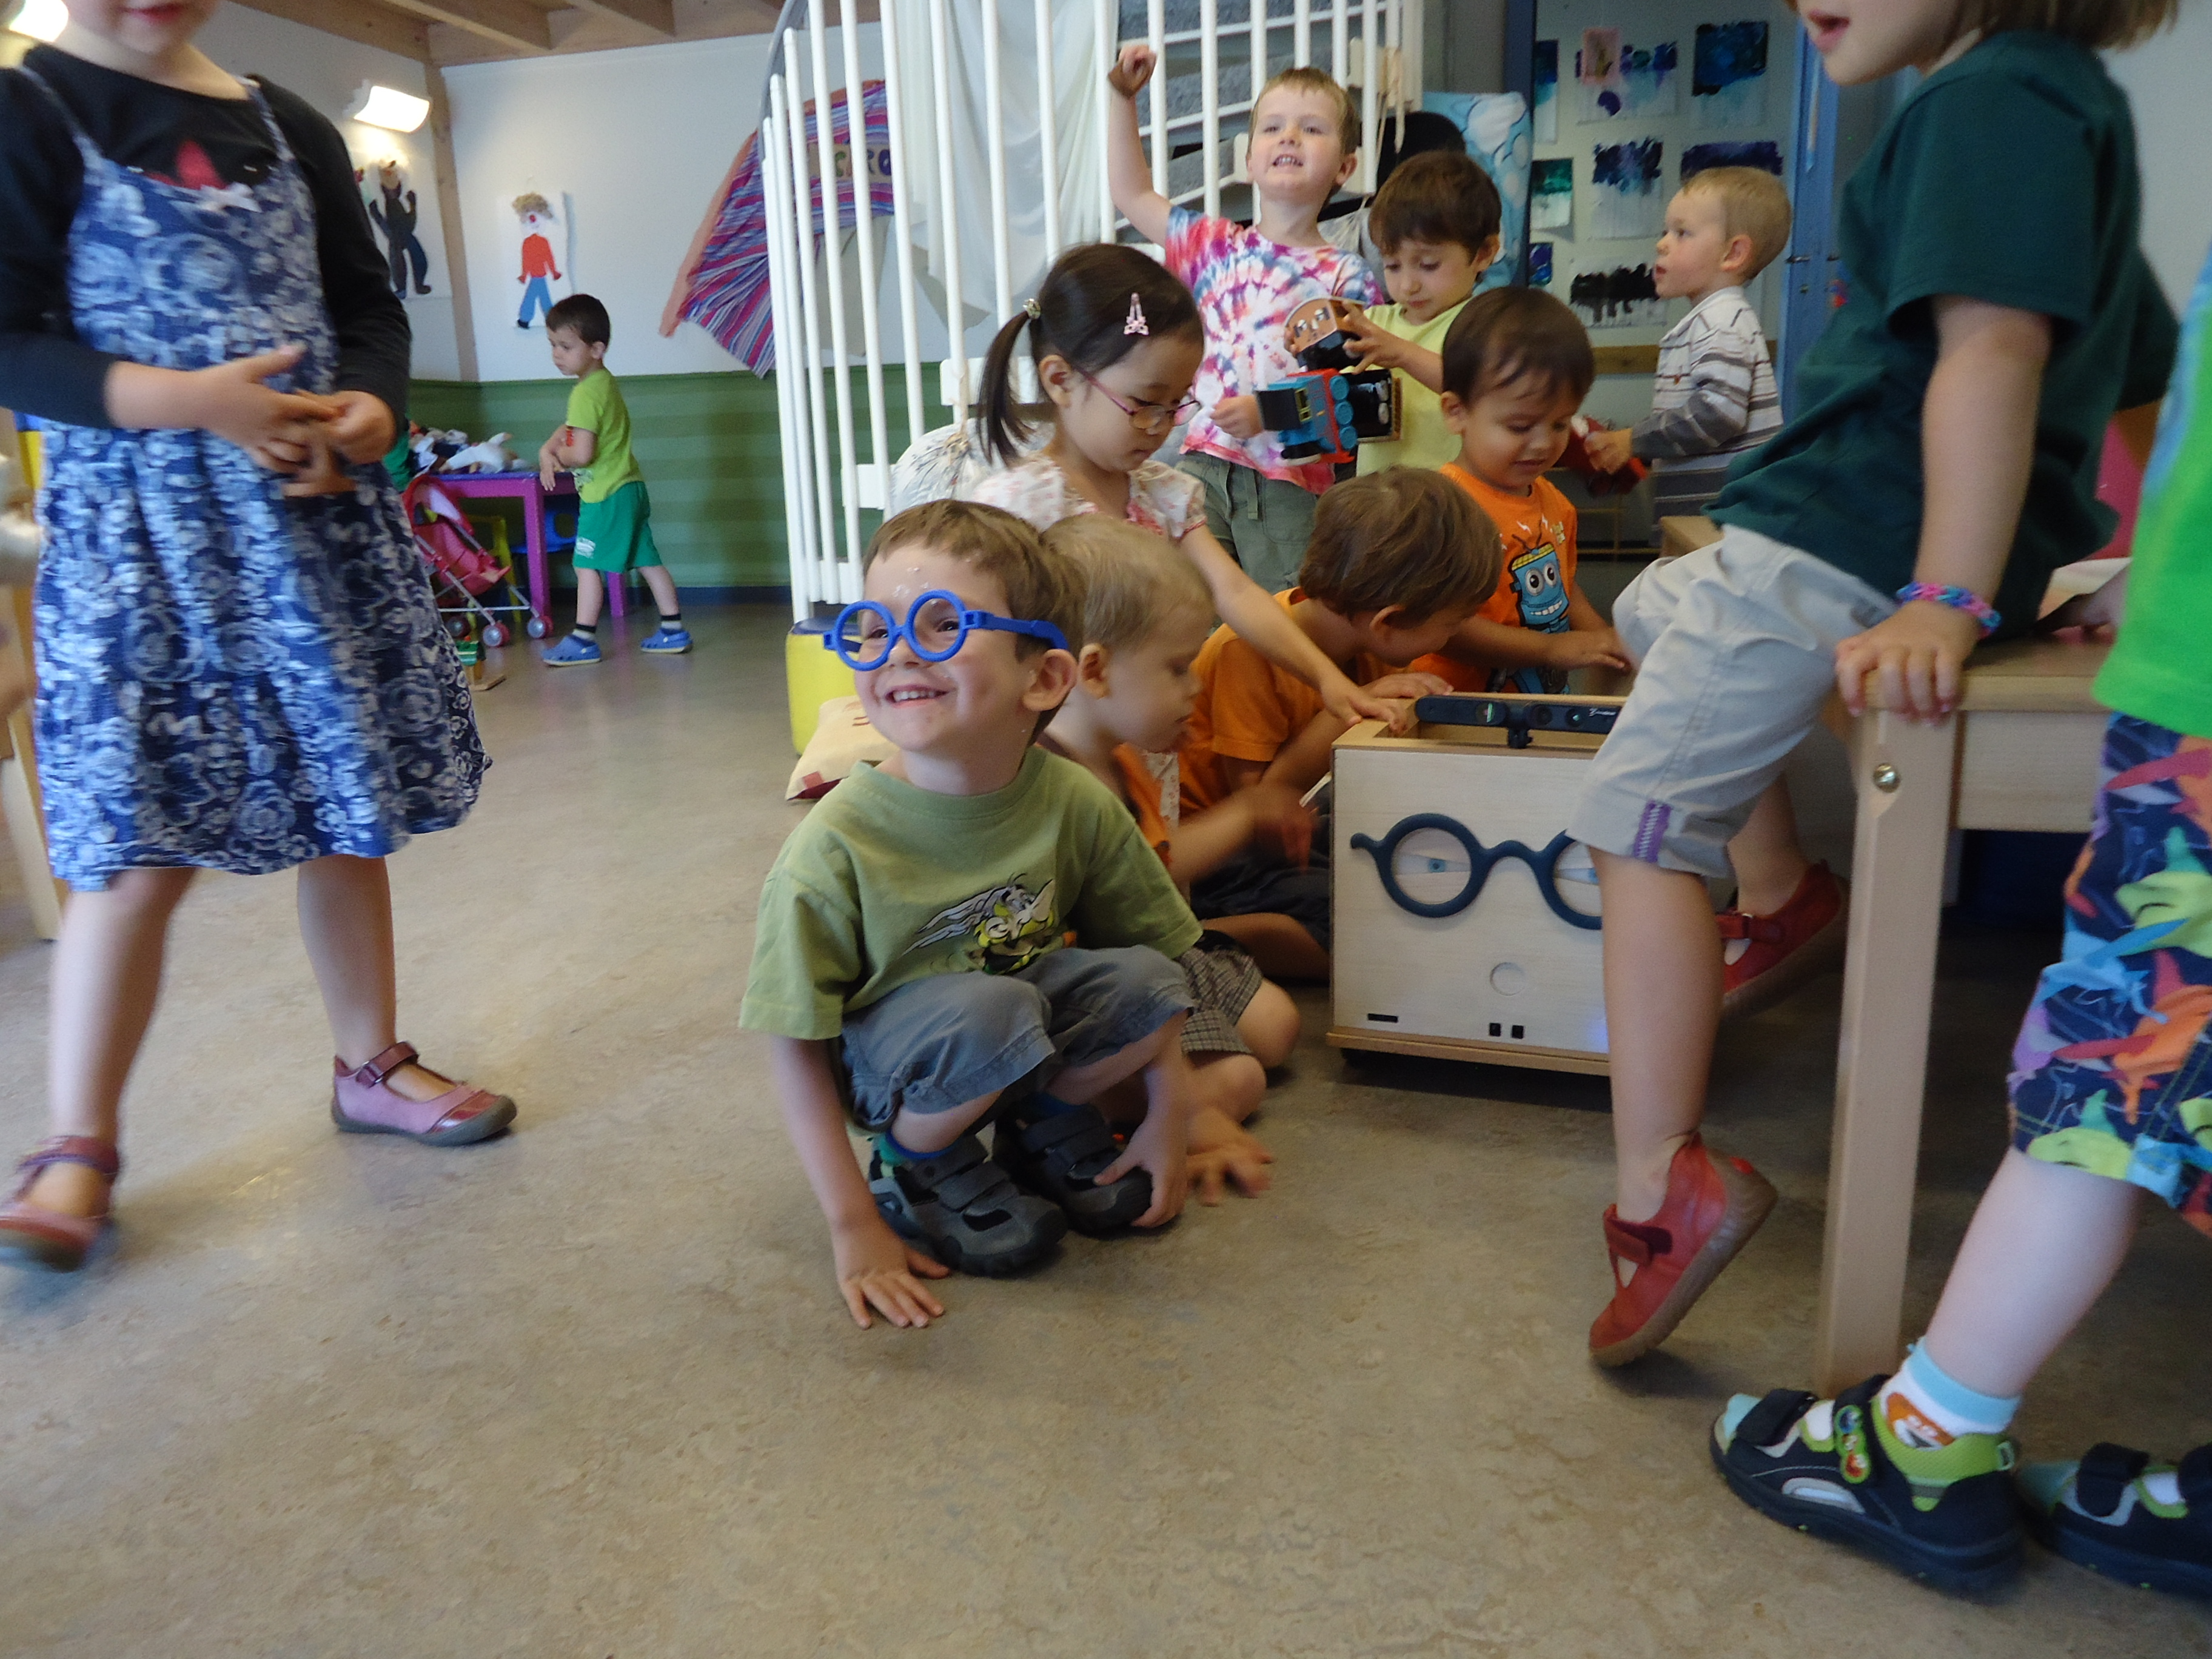
\includegraphics[trim=15cm 0 11cm 0,clip,width=\linewidth]{ranger/ranger_funny_glasses}
            \end{center}
        \end{column}
    \end{columns}

    %    \pause
    %    How to balance long-term \emph{social autonomy} (goal-driven architecture)
    %    with \emph{human oversight}?

\end{frame}

\begin{frame}{KEY SCIENTIFIC AIMS}

    \begin{enumerate}
        \scriptsize
        \item beyond state-of-art \textbf{robust real-world social modelling}; \textbf{social embeddings}
        \item \textbf{public-in-the-loop} approach to design of \textbf{intrinsic social motivation}
        \item \textbf{generative social behaviours} for robots
        \item \textbf{cognitive architecture} for \textbf{long-term interaction}
    \end{enumerate}

    \begin{center}
        %        \resizebox{\linewidth}{!}{
        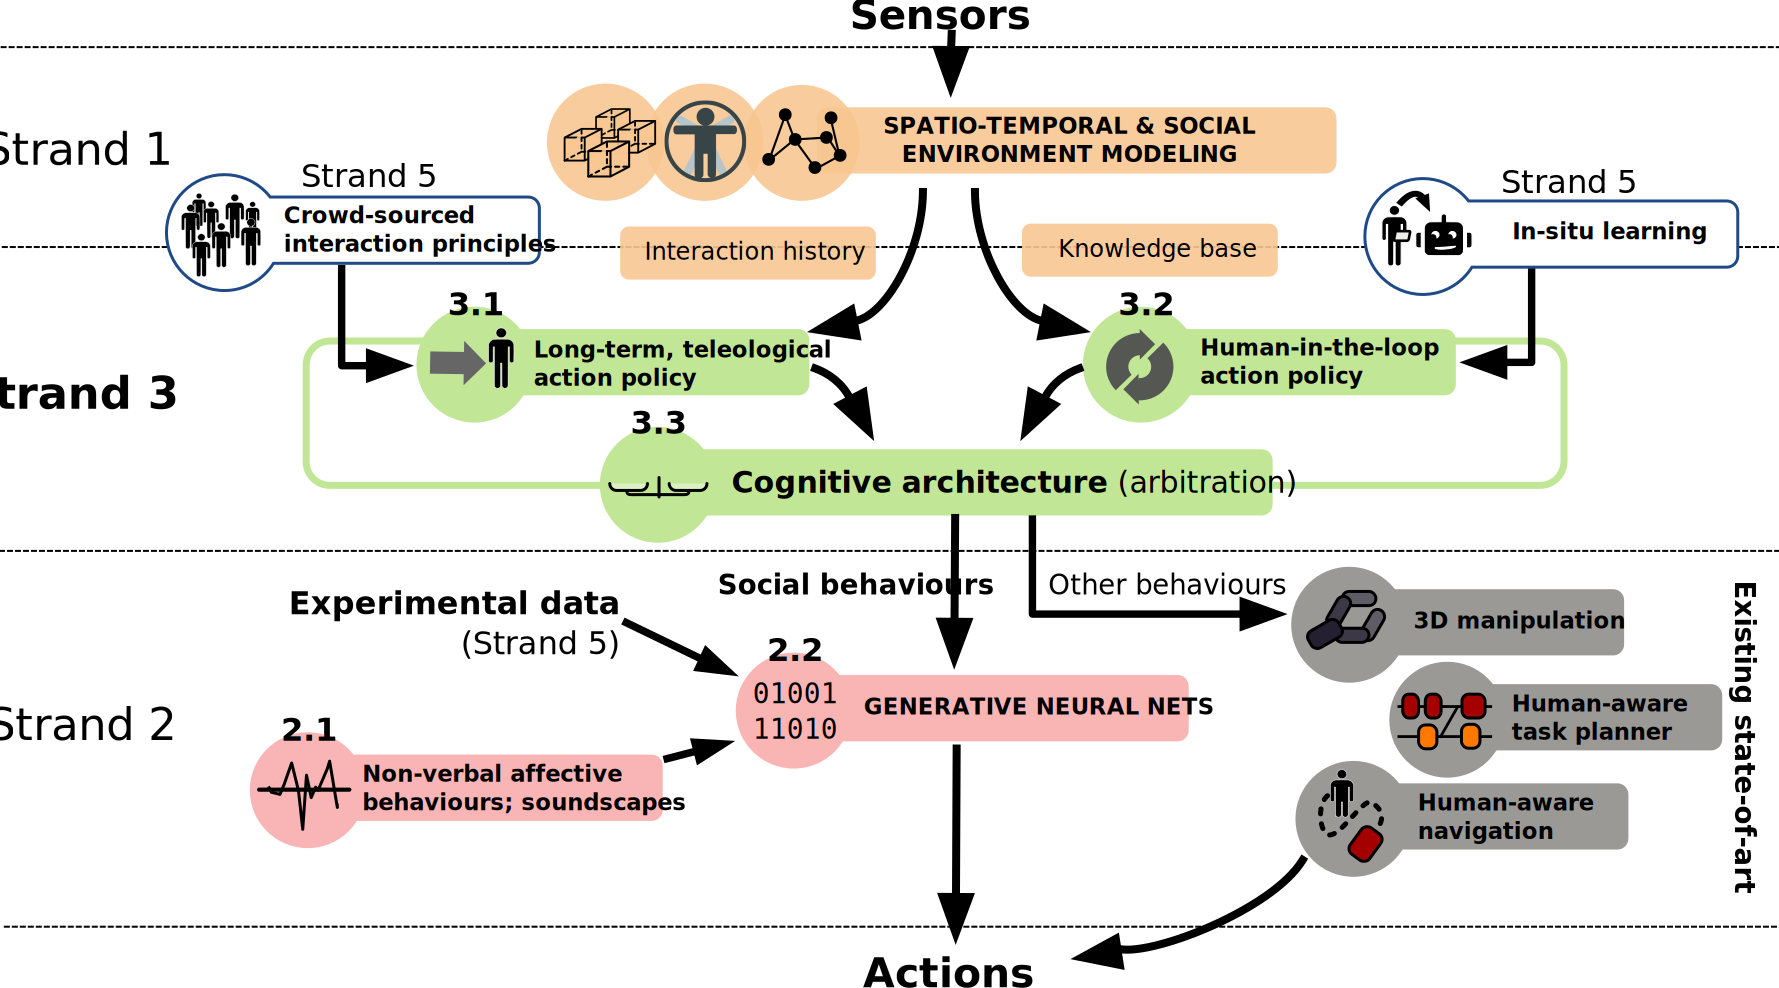
\includegraphics[width=0.7\linewidth]{architectures/archi.pdf}
        %        \hspace{1em}
        %    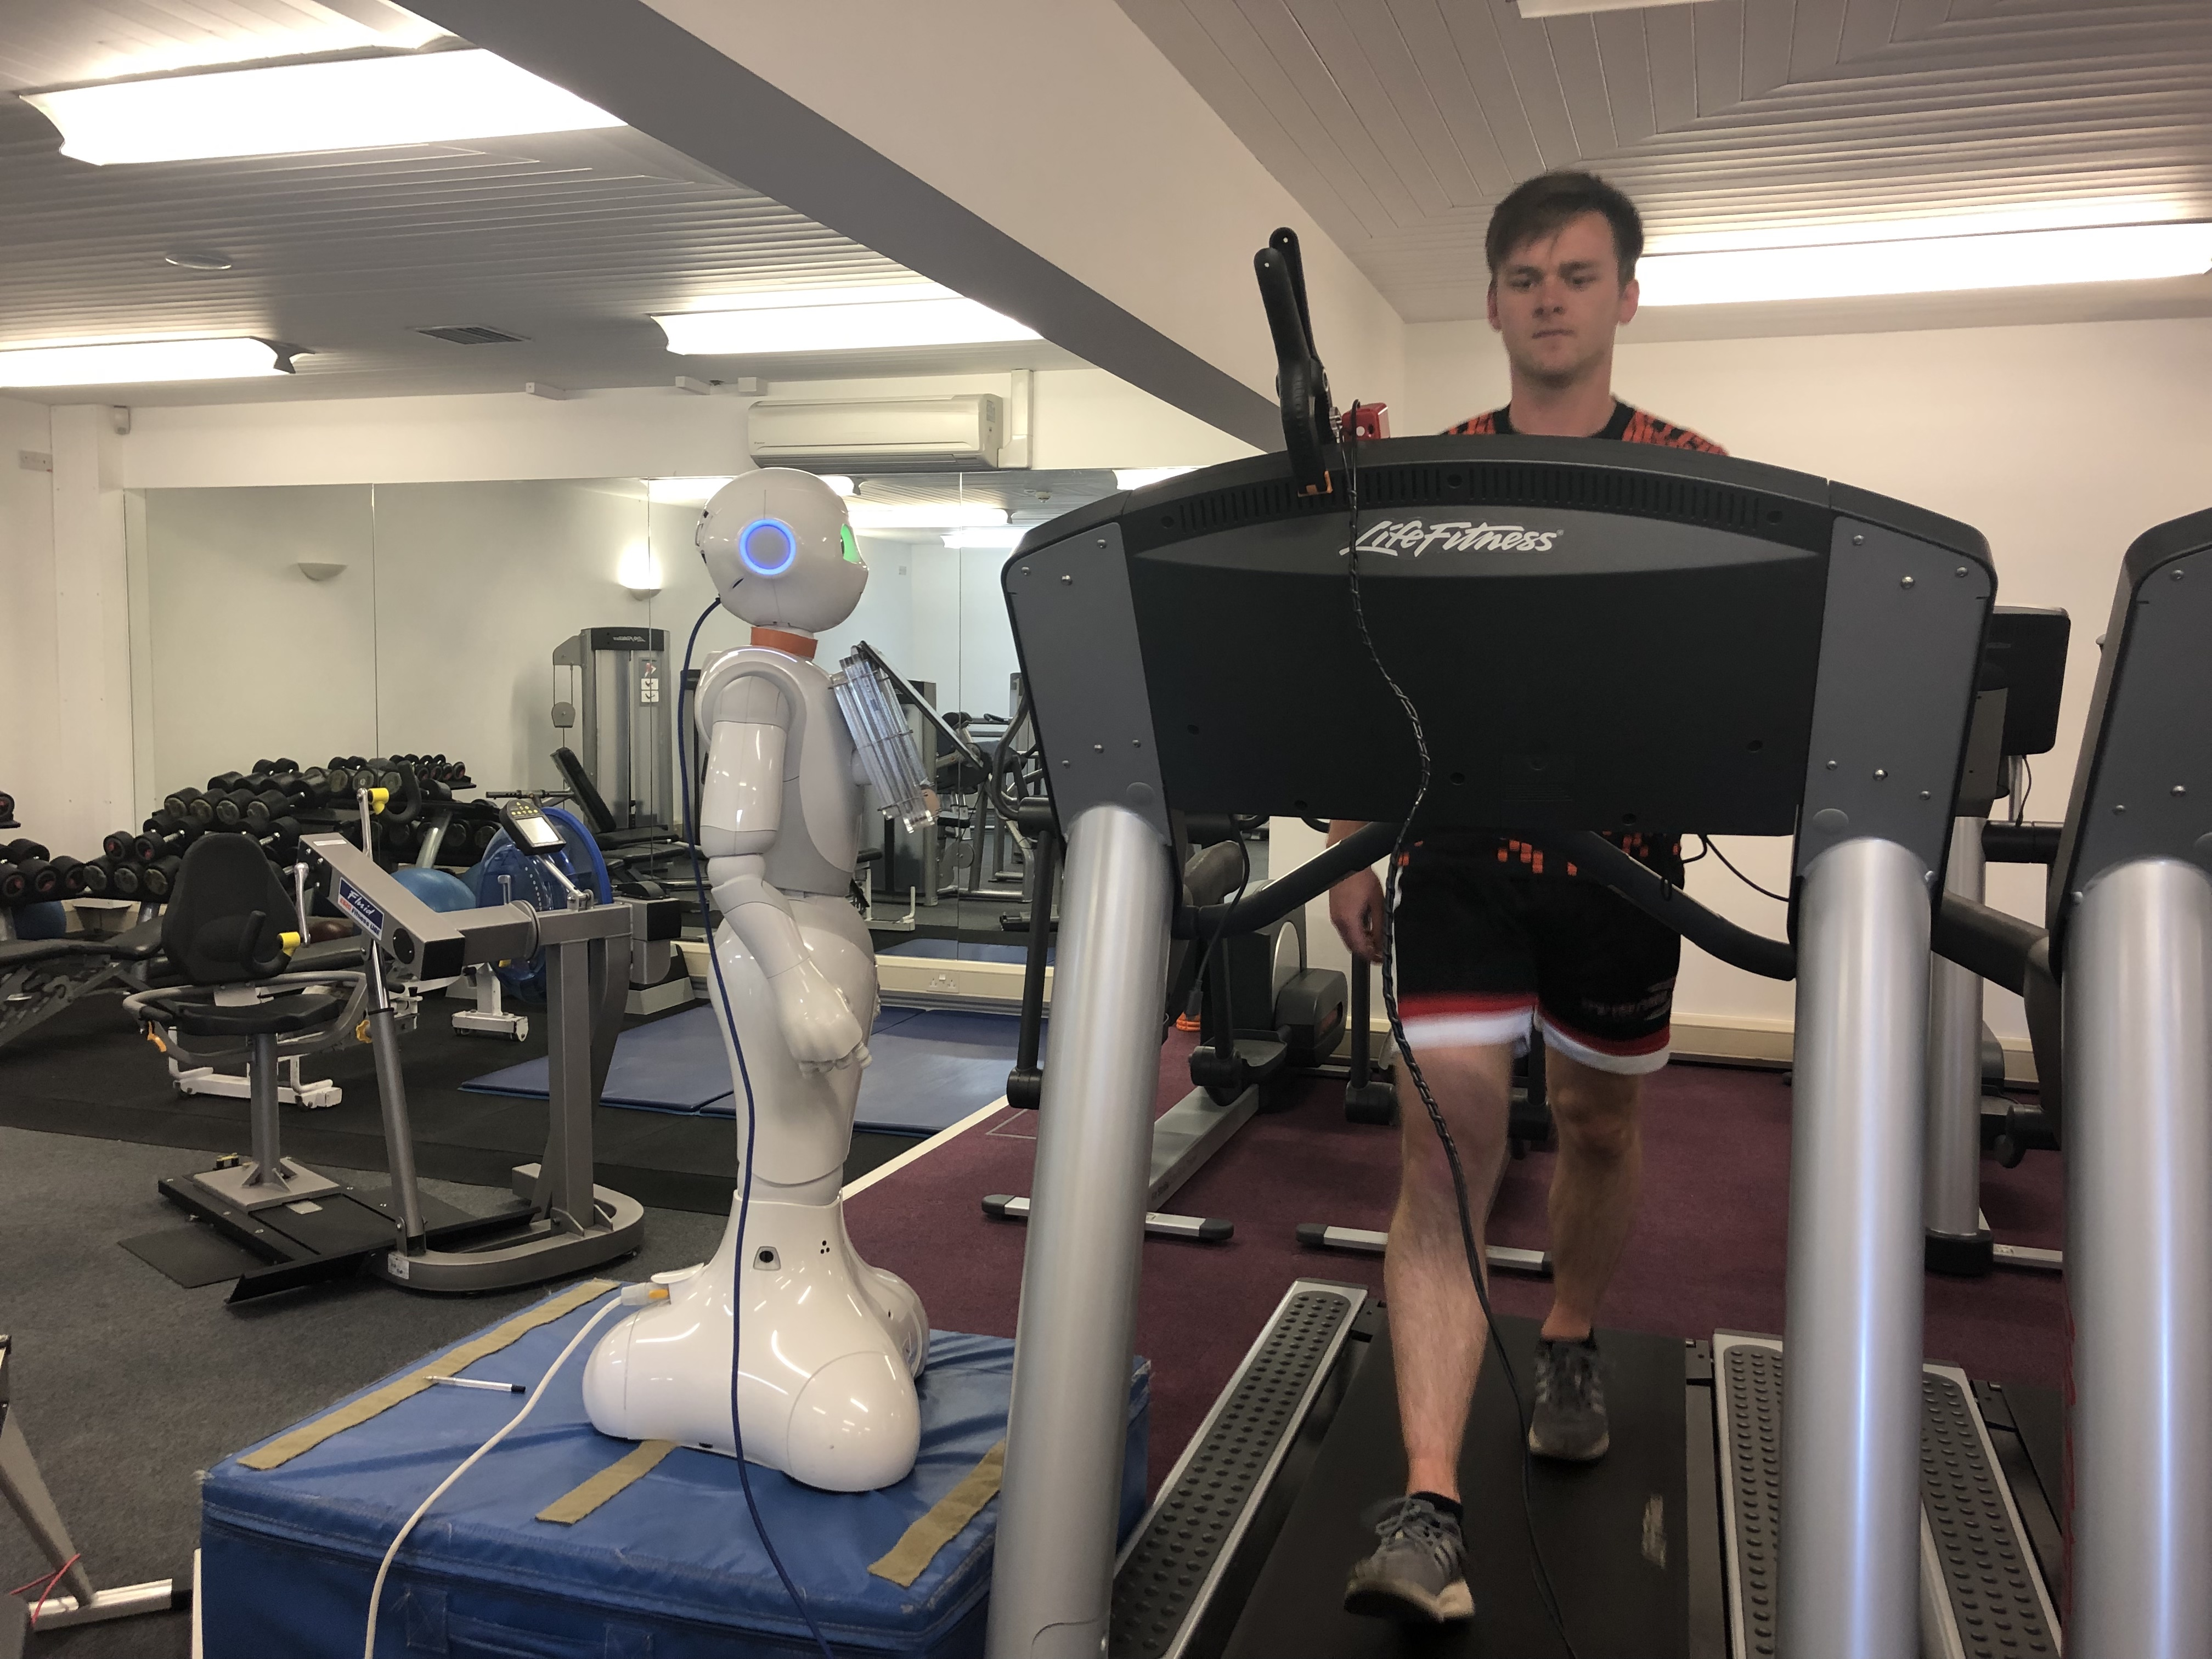
\includegraphics[trim=4cm 0 3cm 0,clip,width=0.25\linewidth]{couch25k/hri.jpg}
        %}
    \end{center}
\end{frame}



%\begin{frame}[label=researchquestion]{}
%
%    \begin{center}
%
%    \Large
%    \bf How to push the state-of-the-art in social robotics?
%
%    \end{center}
%
%    \begin{itemize}
%        \item open, underspecified situations; rich semantics
%            \begin{itemize}
%                \item $\rightarrow$ better spatio-temporal semantic modeling
%            \end{itemize}
%        \item complex social dynamics
%            \begin{itemize}
%                \item $\rightarrow$ \textbf{social situation assessment} 
%            \end{itemize}
%        \item diversity of tasks; long term, sustained interactions
%            \begin{itemize}
%                \item $\rightarrow$ \textbf{goal-driven, non-repetitive
%                    behaviours}
%            \end{itemize}
%    \end{itemize}
%
%
%    \begin{itemize}
%        \item<2-> social acceptability
%        \item<2-> responsible AI
%            \begin{itemize}
%                \item<2-> $\rightarrow$ \textbf{public-in-the-loop} research
%                    
%            \end{itemize}
%    \end{itemize}
%
%
%
%\end{frame}

%\imageframe[scale=0.9]{architectures/sense-plan-act}
%\imageframe[scale=0.9]{architectures/sense-plan-act-2}
%\imageframe[scale=0.9]{architectures/sense-plan-act-3}

%\begin{frame}{}
%    \begin{center}
%        \includegraphics<1>[width=\linewidth]{architectures/sense-plan-act}
%        \includegraphics<2>[width=\linewidth]{architectures/sense-plan-act-2}
%        \includegraphics<3>[width=\linewidth]{architectures/sense-plan-act-3}
%    \end{center}
%\end{frame}


%
%\begin{frame}[plain]
%    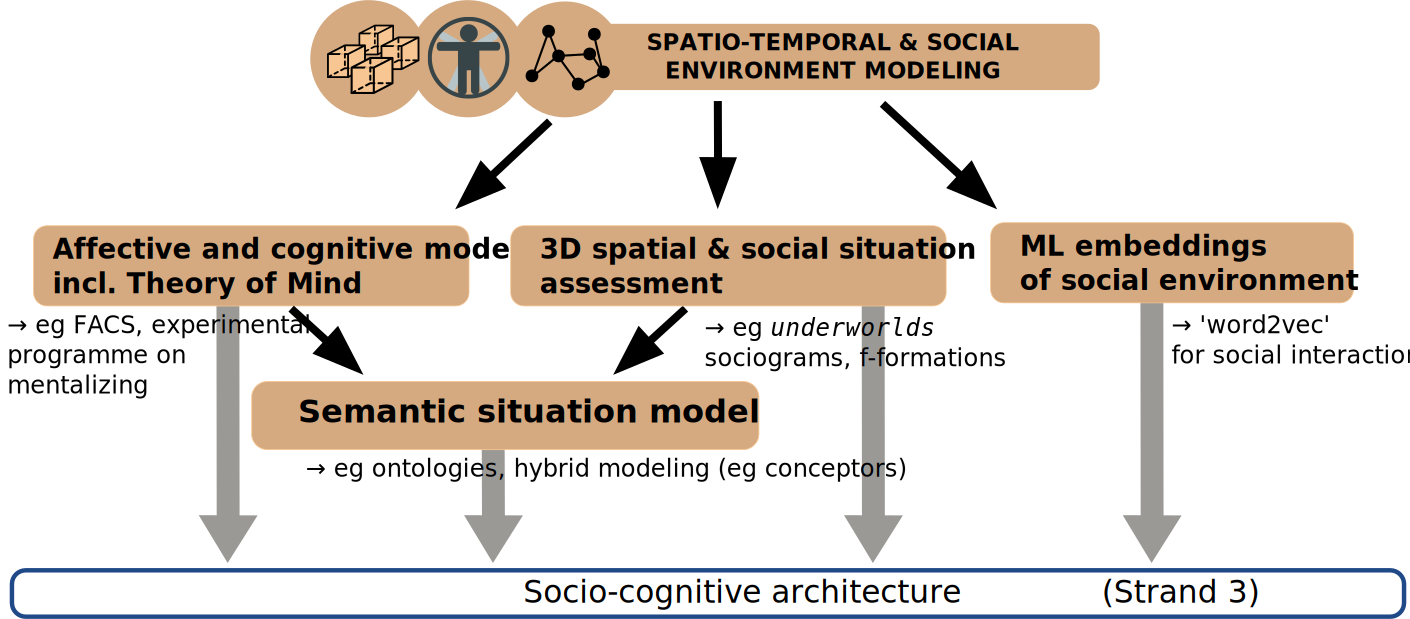
\includegraphics[width=\columnwidth]{architectures/strand1.pdf}
%
%    \vspace{1em}
%    \begin{columns}
%        \begin{column}{0.4\linewidth}
%        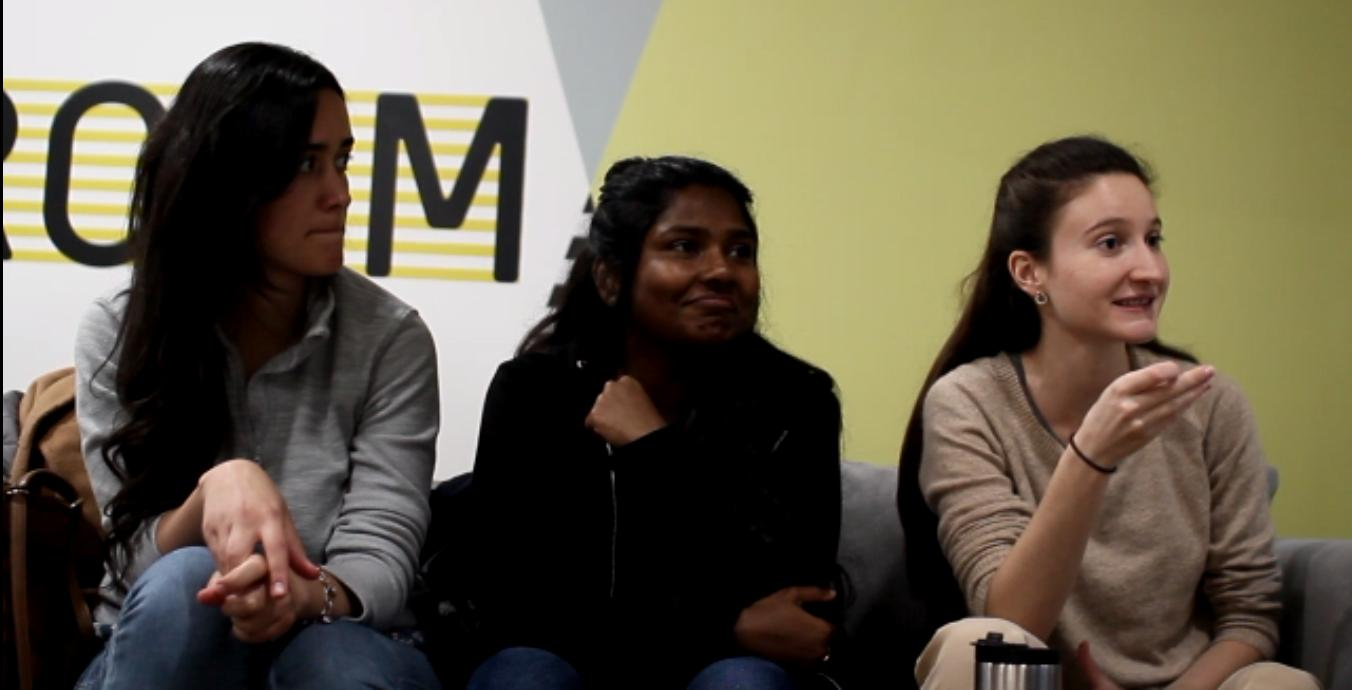
\includegraphics[width=\columnwidth]{social-interactions/social.jpg}
%
%        \end{column}
%        \begin{column}{0.7\linewidth}
%            \scriptsize
%            \begin{itemize}
%                \item SotA machine learning: \textbf{attention nets};
%                    \textbf{deep graph nets}
%                \item \textbf{Social embeddings}: learn an encoding of social
%                    interactions
%                \item \textbf{hybrid pipeline}: eg \emph{conceptors} to build symbolic
%                    models from neural nets 
%                \item real-world \textbf{robustness}: algorithmic redundancy; soft. eng.
%                    expertise (going beyond throw-away research code)
%            \end{itemize}
%
%        \end{column}
%    \end{columns}
%\end{frame}
%
%%\againframe<3>{wps}
%
%
%\begin{frame}[plain]
%
%    \centering
%    \begin{columns}
%        \begin{column}{0.6\linewidth}
%            \centering
%            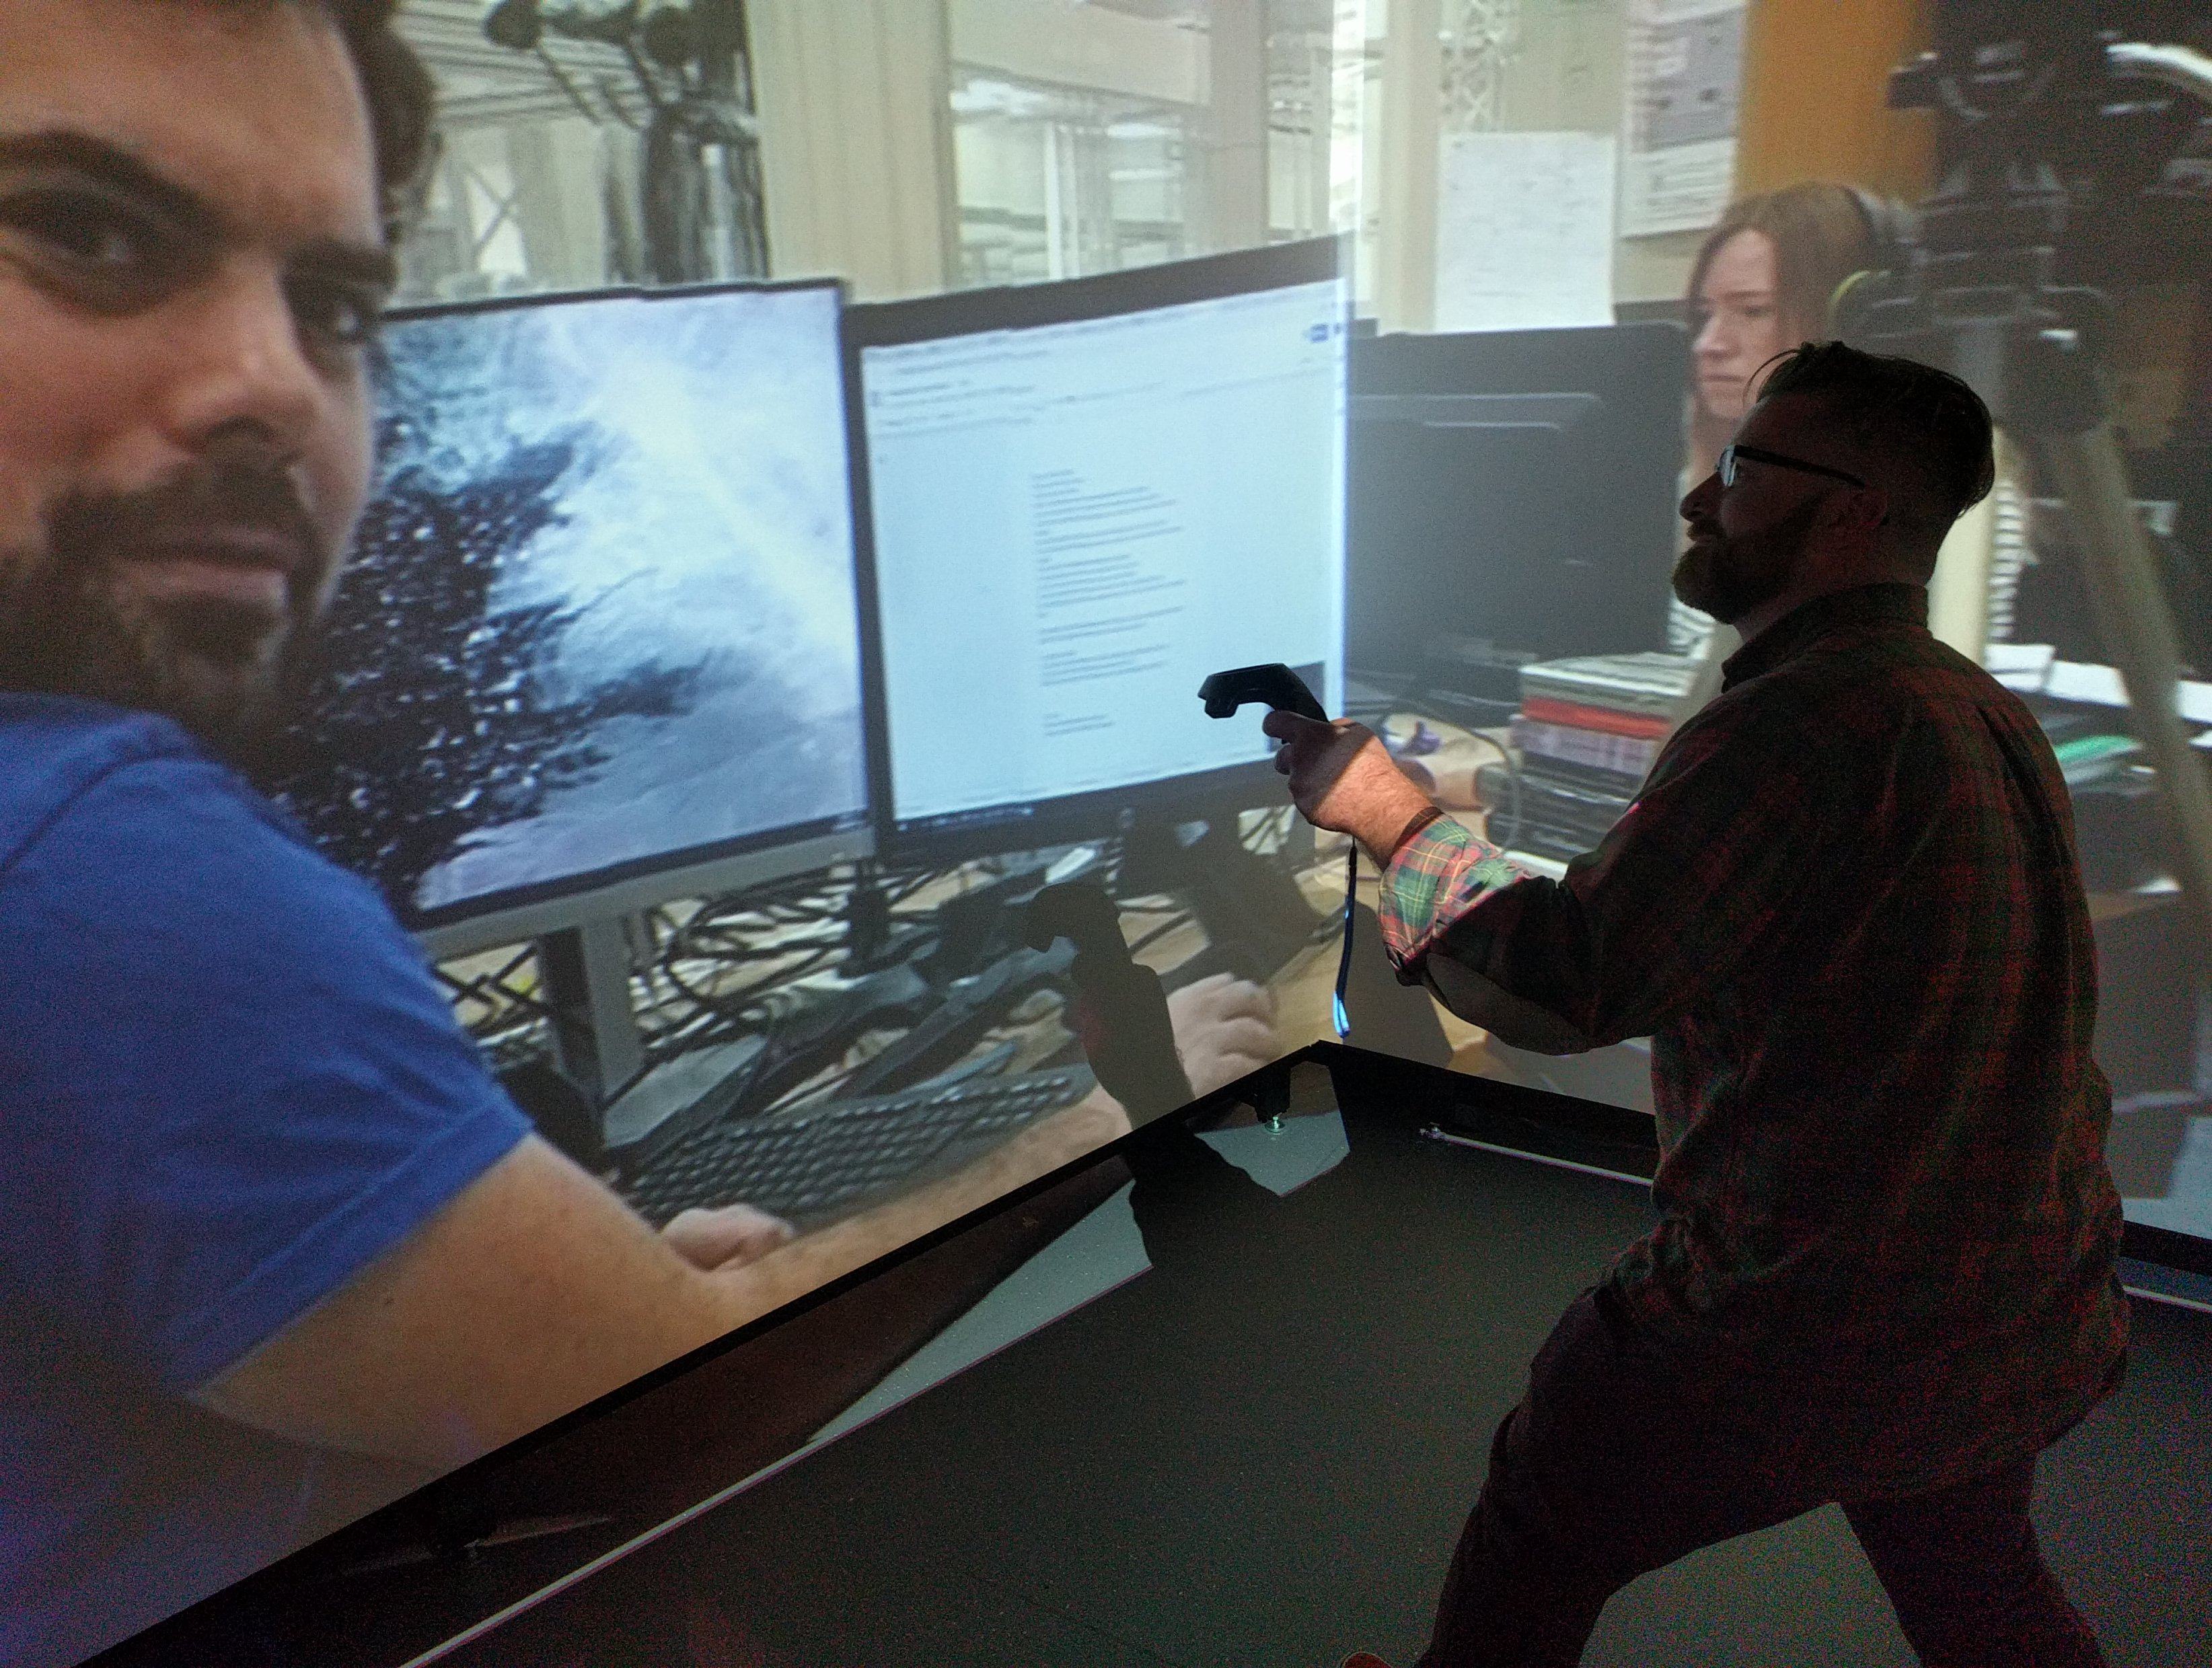
\includegraphics[width=\linewidth]{generative-behaviours/immersive-teleoperation}
%        \end{column}
%        \begin{column}{0.4\linewidth}
%            \centering
%            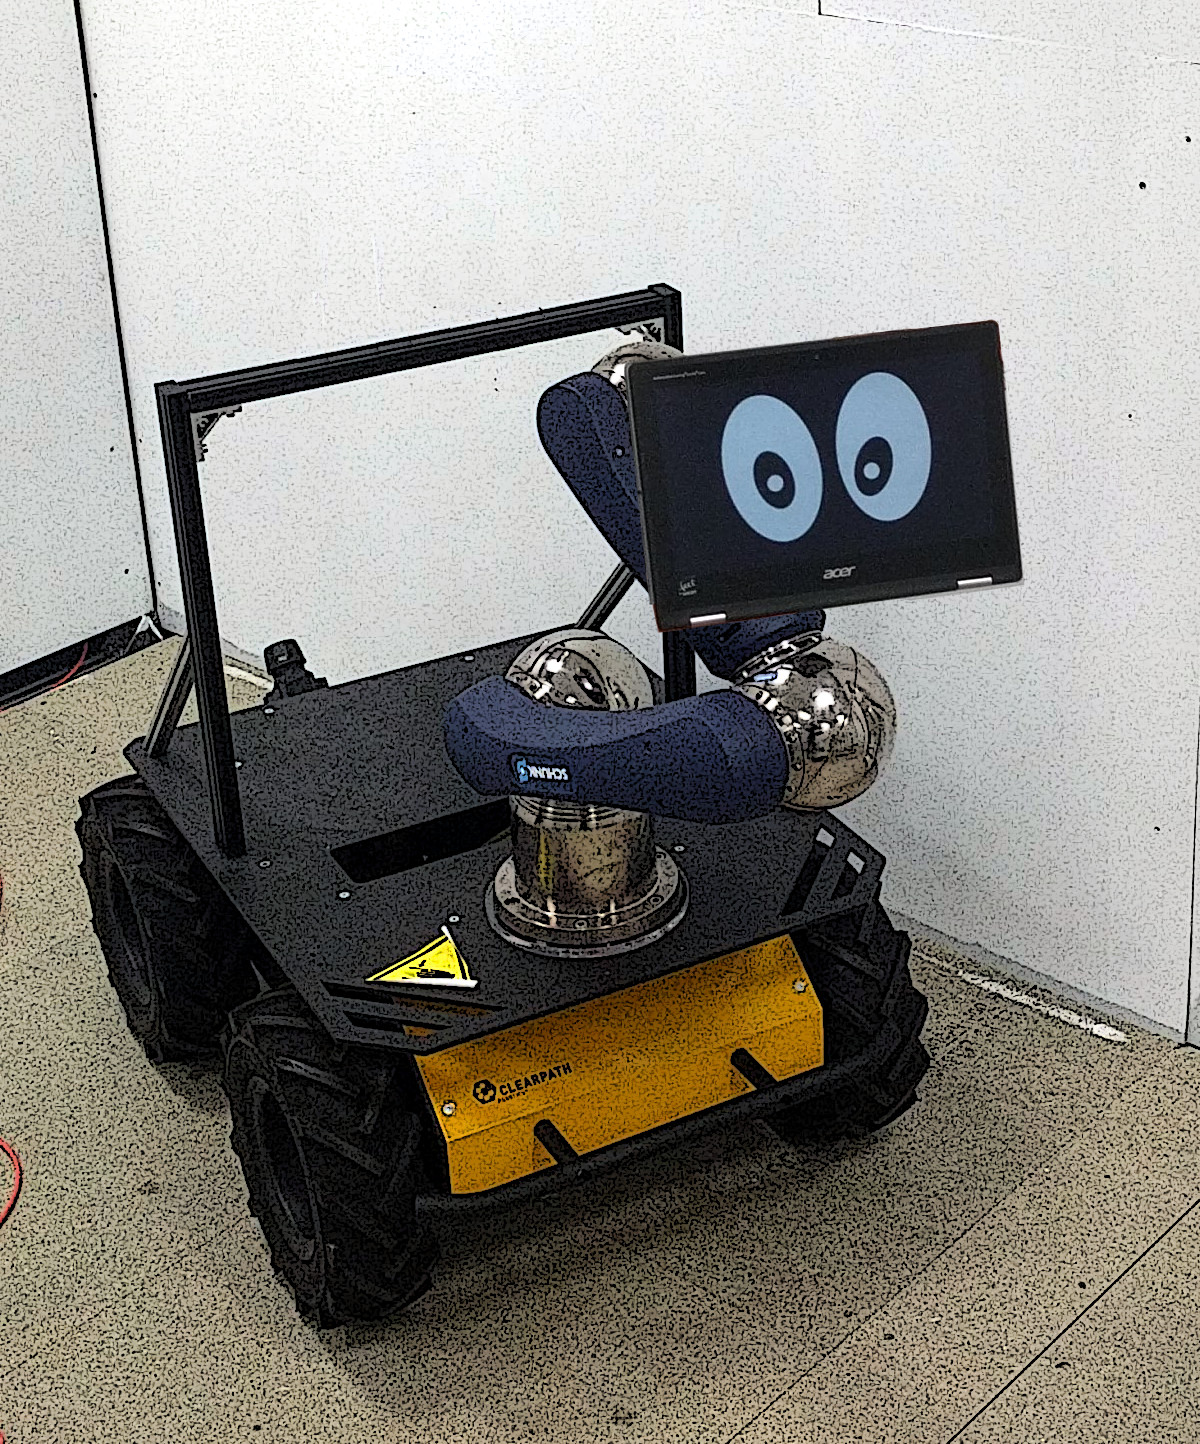
\includegraphics[height=4.9cm]{generative-behaviours/husky}
%        \end{column}
%    \end{columns}
%
%    \vspace{1em}
%
%    \begin{columns}
%        \begin{column}{0.4\linewidth}
%            \centering
%            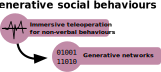
\includegraphics[width=\linewidth]{architectures/strand2}
%        \end{column}
%        \begin{column}{0.6\linewidth}
%
%            \scriptsize
%            \begin{itemize}
%                \item Cracking the `\textbf{non-repetitive, socially congruent}' behaviour
%                    generation problem
%                \item Extend \textbf{Generative Adversarial Networks} \emph{à la} AppGAN to complex
%                    behaviours (re-use \emph{social embeddings})
%                \item \textbf{Immersive technologies} to build datasets
%                \item \textbf{Transdiscplinary approach}, incl. arts: choreographer, sound
%                    expert
%            \end{itemize}
%        \end{column}
%    \end{columns}
%\end{frame}
%
%
%%\againframe<5>{wps}
%
%\begin{frame}<4>[plain]
%    \begin{center}
%    \begin{columns}
%        
%
%        \begin{column}{0.3\linewidth}
%            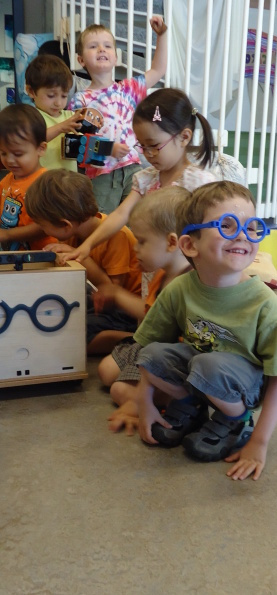
\includegraphics[height=0.75\paperheight]{croquignole-narrow.jpg}
%        \end{column}
%
%
%        \begin{column}{0.7\linewidth}
%            \centering
%            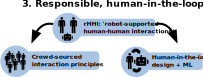
\includegraphics[width=\columnwidth]{architectures/strand4}
%            \vspace{1em}
%
%            \scriptsize
%            \begin{enumerate}
%                \item<1-> interactive reinforcement learning
%                    \begin{itemize}
%                        \item \emph{\scriptsize how to scale it to multiple tasks?}
%                        \item \emph{\scriptsize how to deal with non-trivial semantics?}
%                    \end{itemize}
%                \item<2-> intrinsic social motivation
%                    \begin{itemize}
%                        \item \scriptsize large-scale public engagement to
%                            \textbf{co-design interaction principles: meaningful \& useful social goals}
%                    \end{itemize}
%                \item<3-> responsible AI
%                    \begin{itemize}
%                        \item \scriptsize\textbf{crowd-sourcing social norms} for human-robot
%                            interactions
%                    \end{itemize}
%
%            \end{enumerate}
%            \vspace{1em}
%
%            \onslide<4>{
%            $\rightarrow$ shift from human-robot interactions to \textbf{robot-supported human-human interactions}
%            }
%
%
%        \end{column}
%
%
%    \end{columns}
%    \end{center}
%\end{frame}
%
%\againframe<4>{wps}


\begin{frame}{MIXED METHODS}

    Standard methods:
    \begin{itemize}
        \item Exploratory field work/case studies
        \item Participatory design; co-design
        \item Ecologically-valid controlled studies
        \item Longitudinal studies
        \item Large-scale online crowd-sourcing
    \end{itemize}

    Novel methods that I introduce in my project:
    \begin{itemize}
        \item \textbf{Public-in-the-loop machine learning}
        \item \textbf{Immersive teleoperation and generative behaviours} with artists
    \end{itemize}

\end{frame}

%\begin{frame}{FOCUS: SOCIAL EMBEDDINGS}
%    \begin{columns}
%        \begin{column}{0.5\linewidth}
%    \begin{center}
%        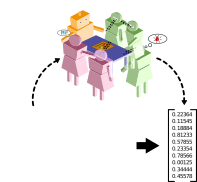
\includegraphics[width=\linewidth]{social-interactions/social-embeddings}
%    \end{center}
%
%        {\scriptsize
%        \textbf{social embeddings}: learning a compact, sub-symbolic representation of social interactions
%        }
%        \end{column}
%        \begin{column}{0.5\linewidth}
%            \begin{itemize}
%                \item real-world social interactions are highly dynamic, noisy,
%                    multi-modal
%                \item hard for the robot to model and reason about
%                \item $\rightarrow$ \textbf{learn an embedding}: Attention nets, Deep
%                    graph nets
%                \item can be used by the robot to \textbf{recognise social situation} and
%                    \textbf{generate congruent social behaviours}
%            \end{itemize}
%        \end{column}
%    \end{columns}
%\end{frame}
%
%\begin{frame}{FOCUS: HUMAN-IN-THE-LOOP ACTION POLICIES}
%    \begin{center}
%        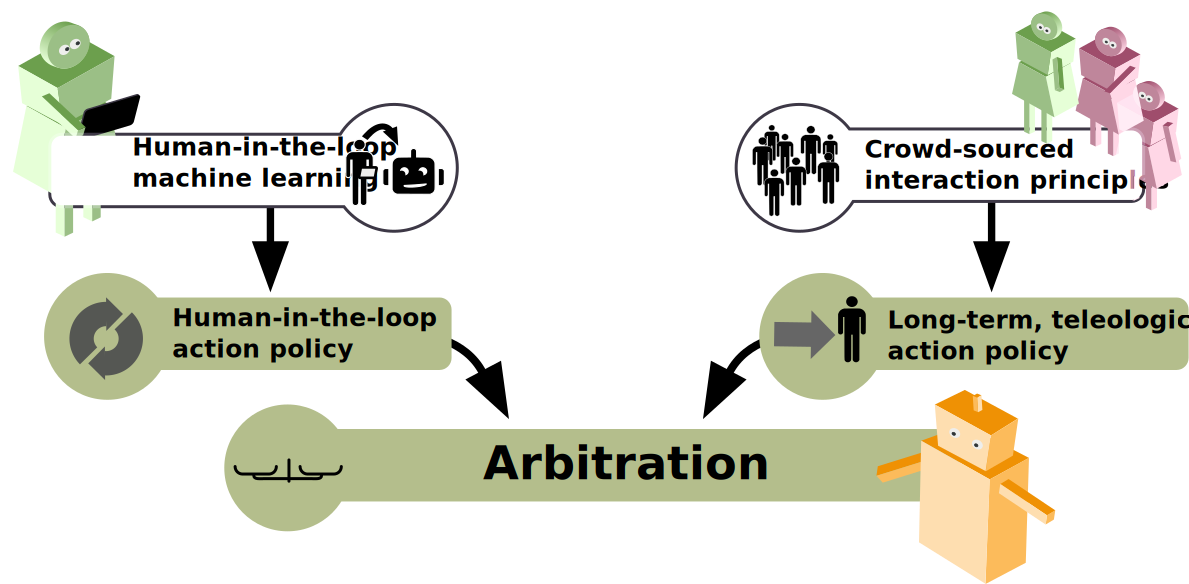
\includegraphics[width=0.8\linewidth]{architectures/arbitration}
%    \end{center}
%
%    \begin{itemize}
%            \scriptsize
%        \item \textbf{end-users and public to play a key role}:
%        \item \textbf{crowd-sourced pro-social goals} (eg `show attention', `appear
%            alive') drives long-term behaviours
%        \item \textbf{short-term/domain-specific policies learned} via
%            interactive reinforcement learning (IRL)
%        \item \textbf{cognitive arbitration} between the two, based on
%            \textbf{experience transfer}
%    \end{itemize}
%\end{frame}

\begin{frame}<1>[label=wps]{4 AXES TO SCAFFOLD A RESEARCH GROUP}
    \begin{center}
    \only<1>{
        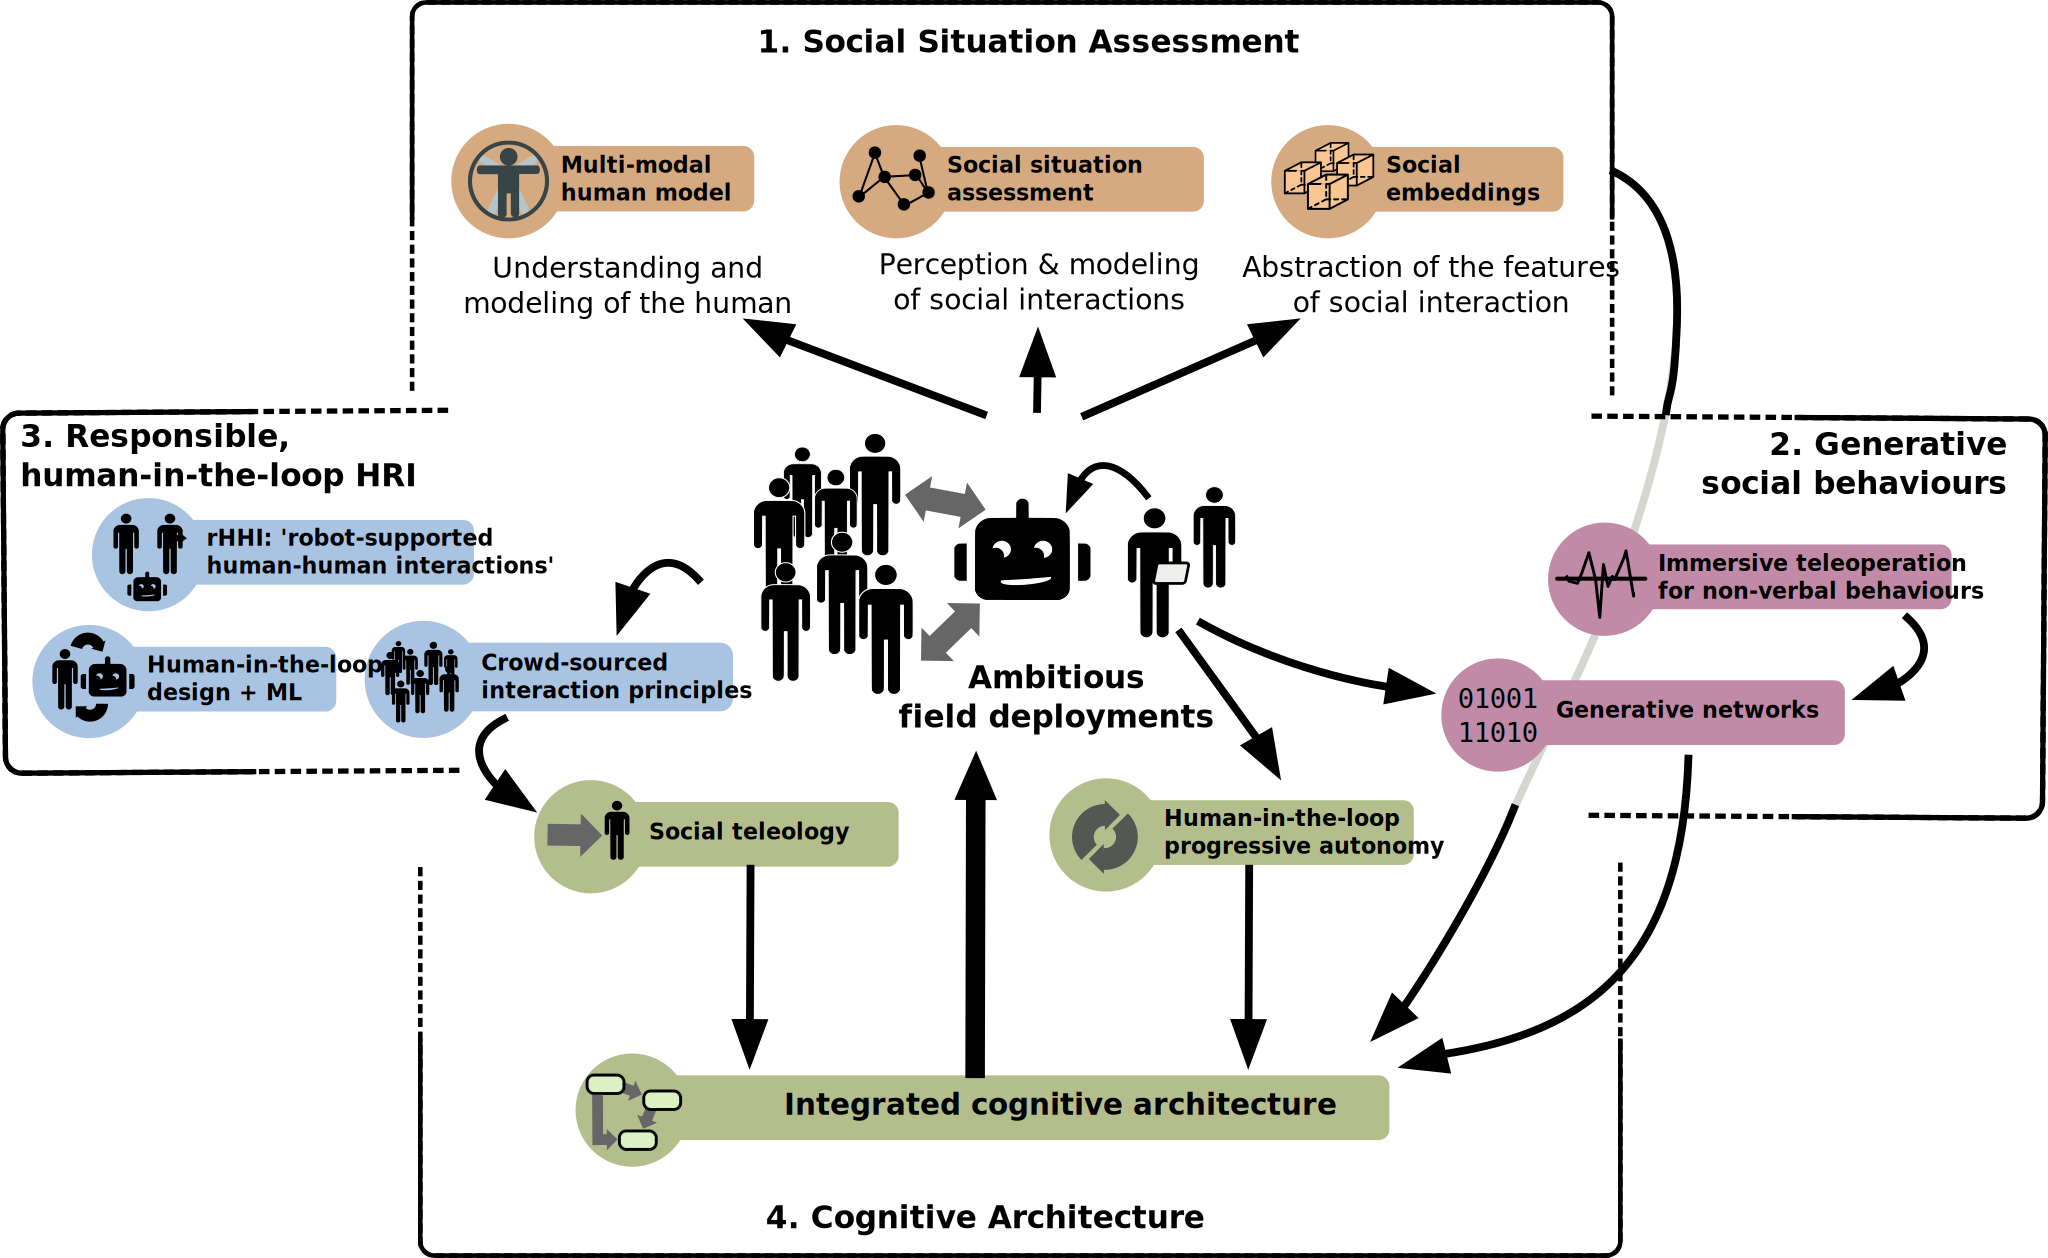
\includegraphics[width=\linewidth]{architectures/wps}
    }
    \only<2>{
        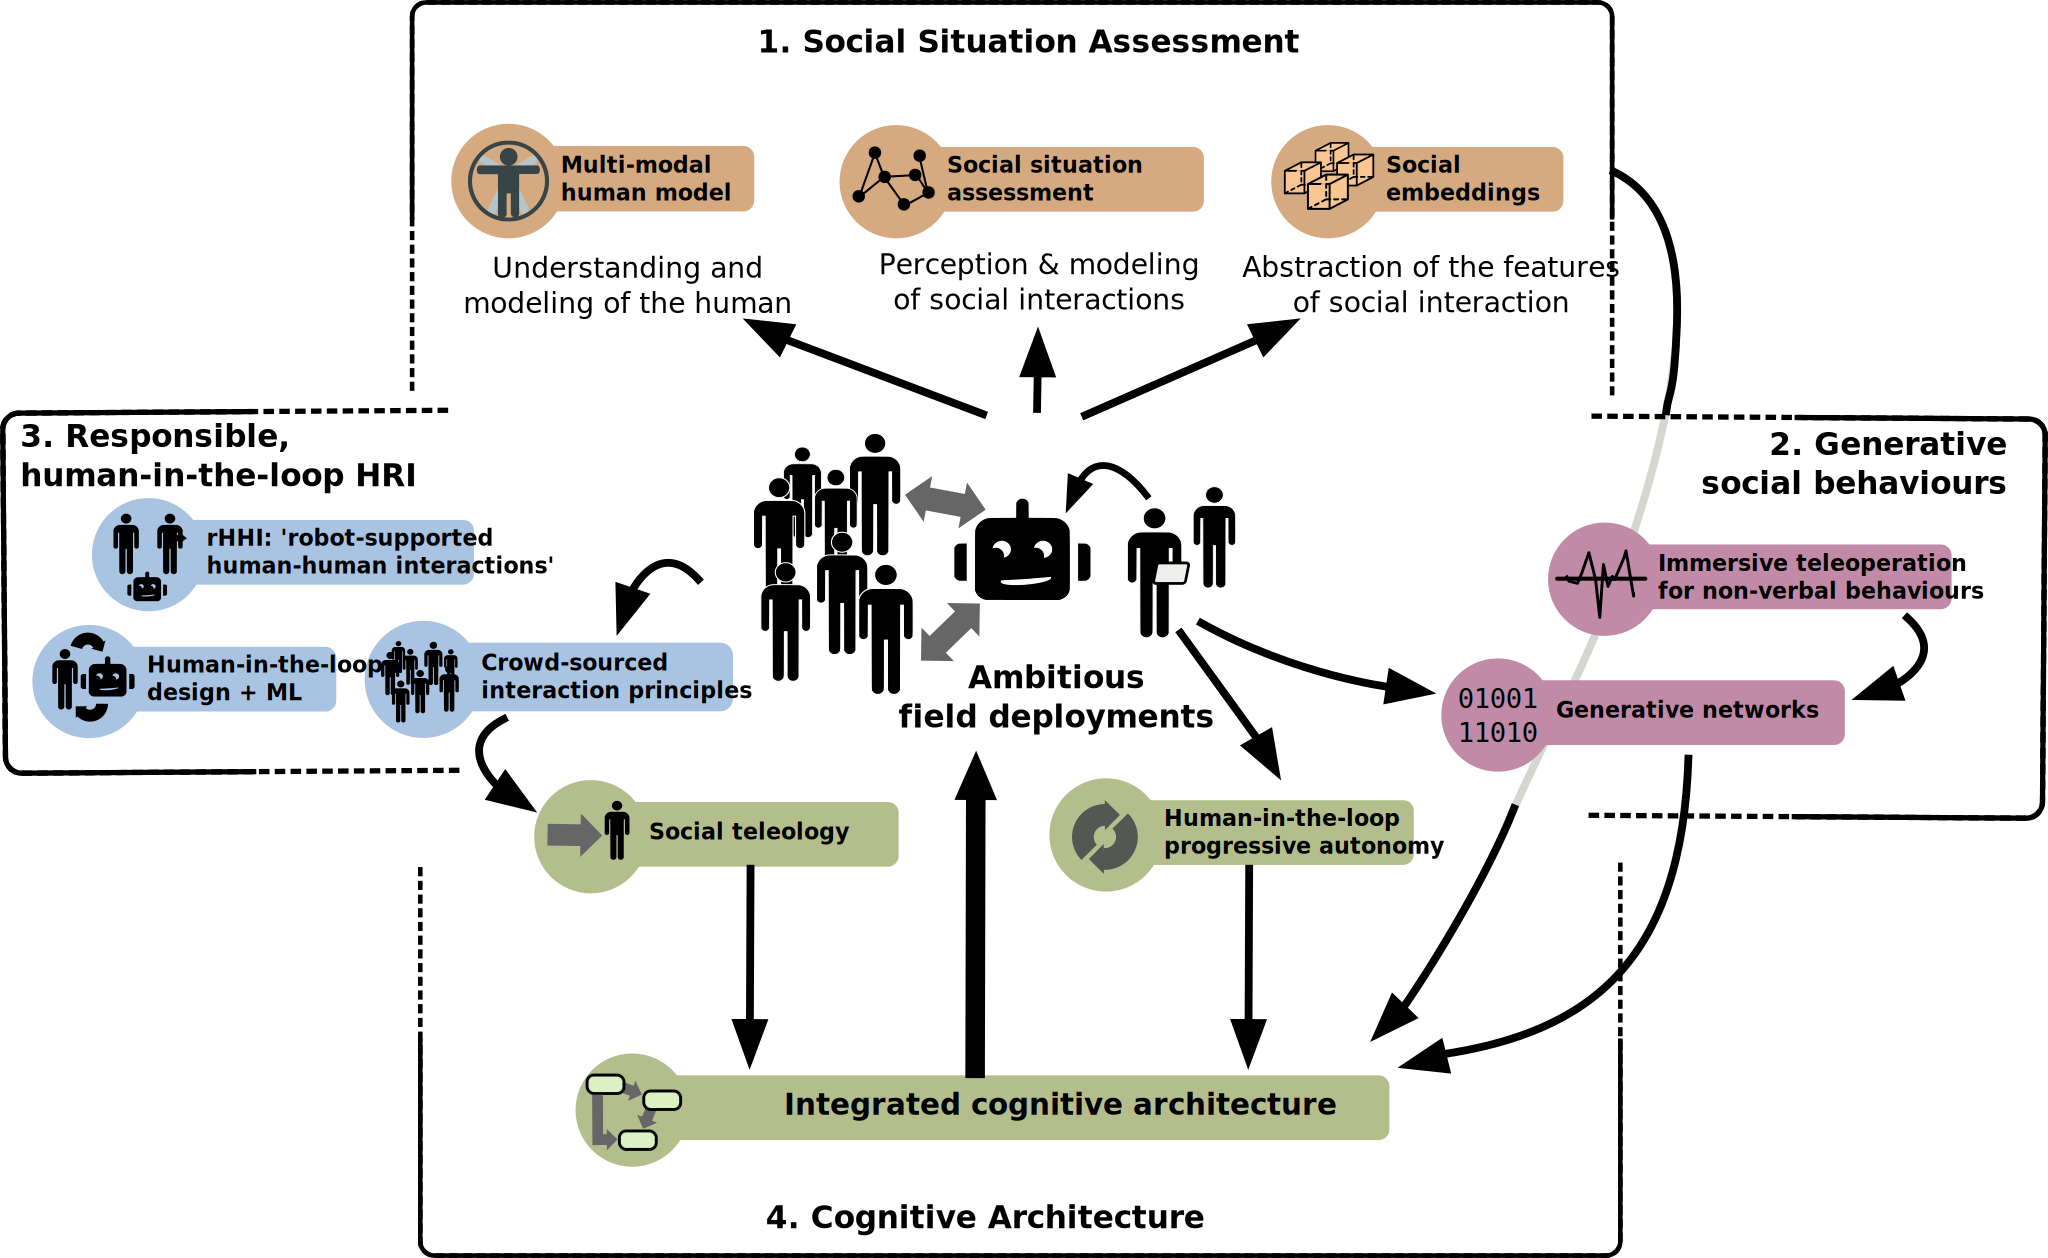
\includegraphics[trim=8cm 20cm 8cm 0,clip,width=\linewidth]{architectures/wps}
    }
    \only<3>{
        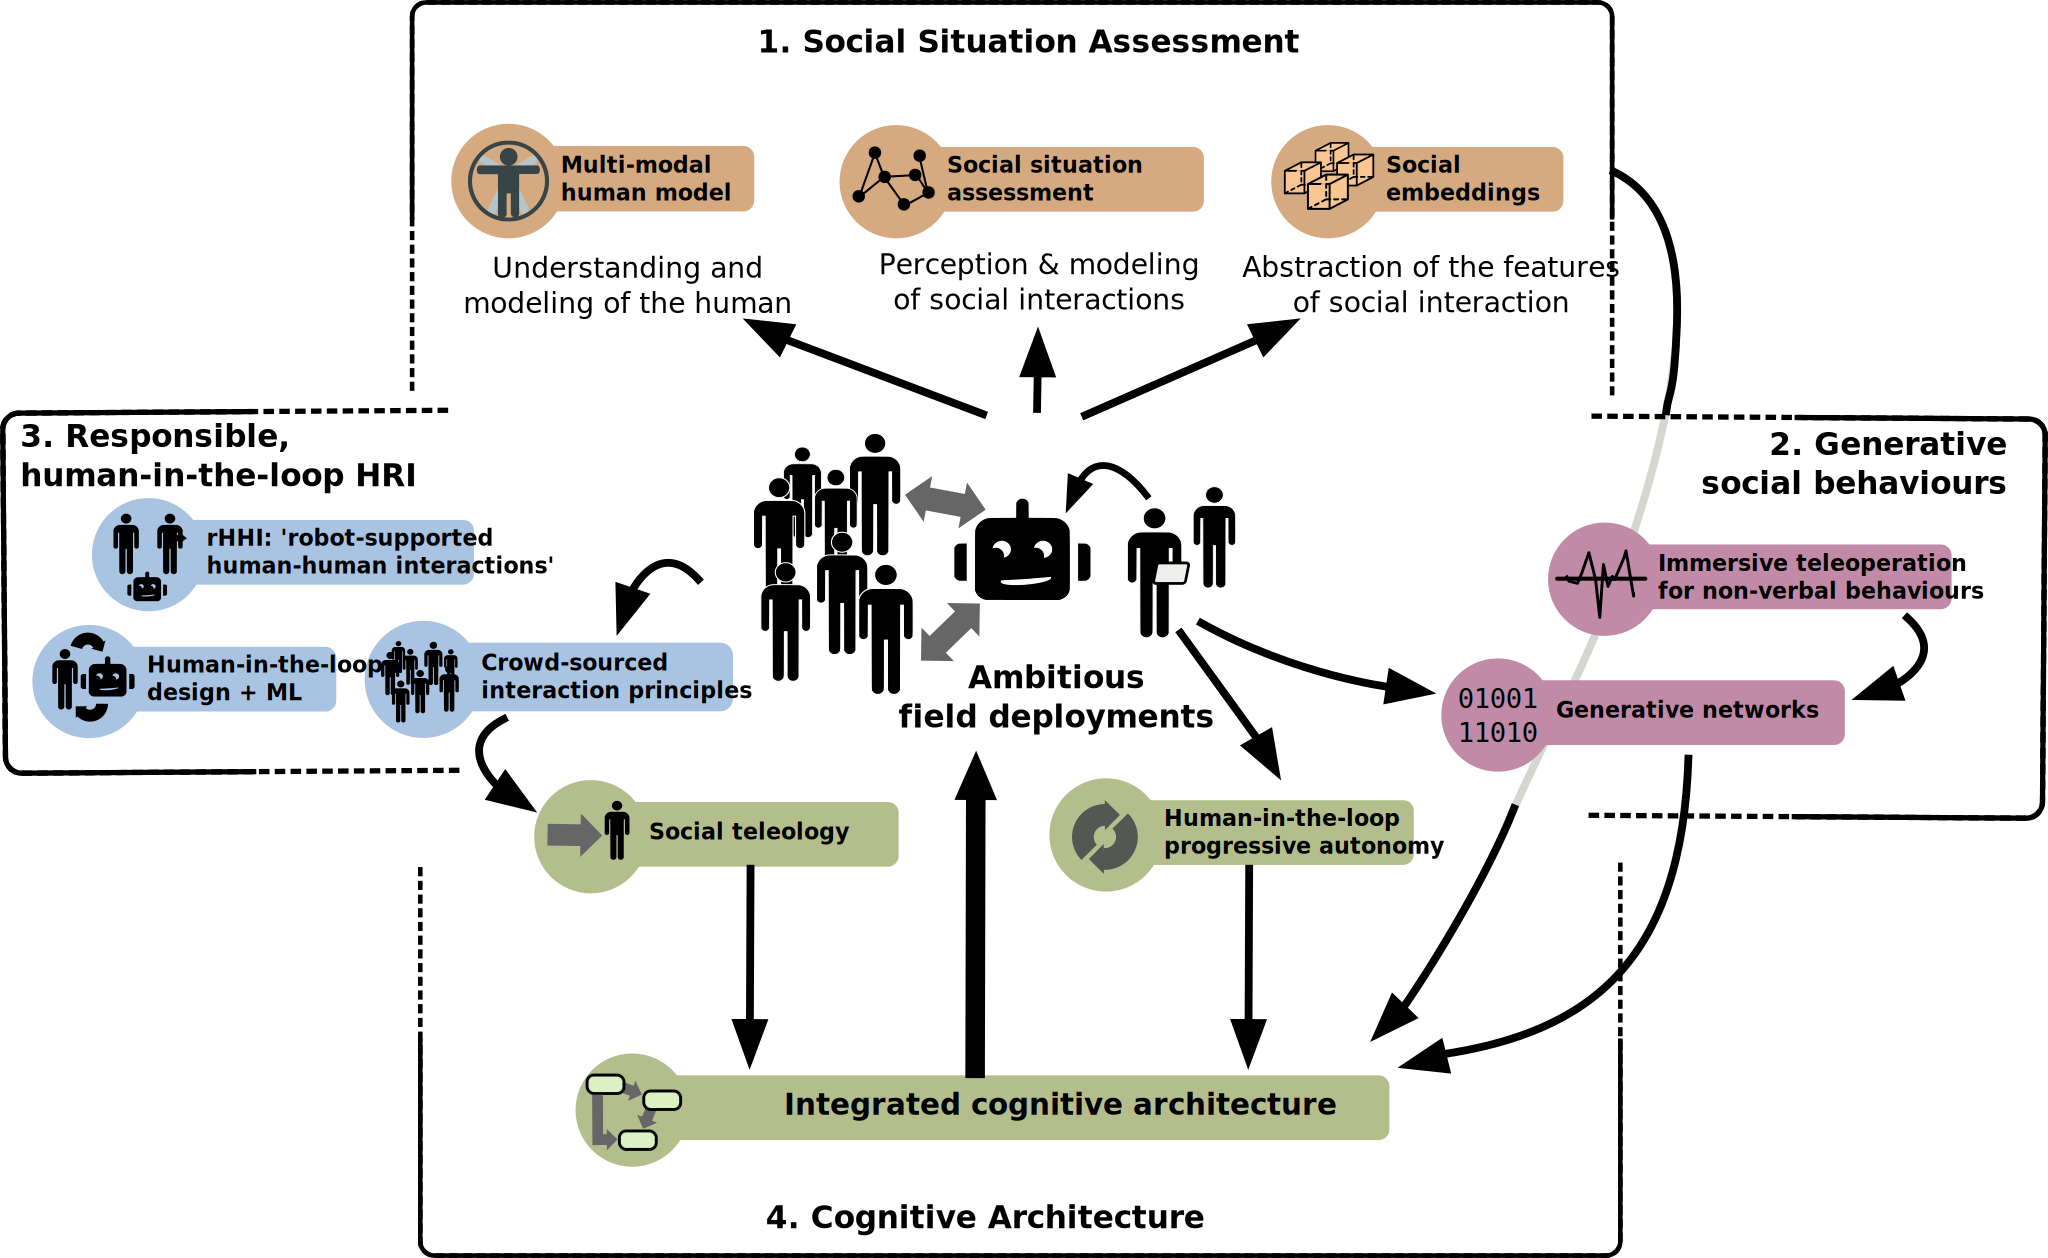
\includegraphics[trim=30cm 8cm 0 8cm,clip,width=0.7\linewidth]{architectures/wps}
    }
    \only<4>{
        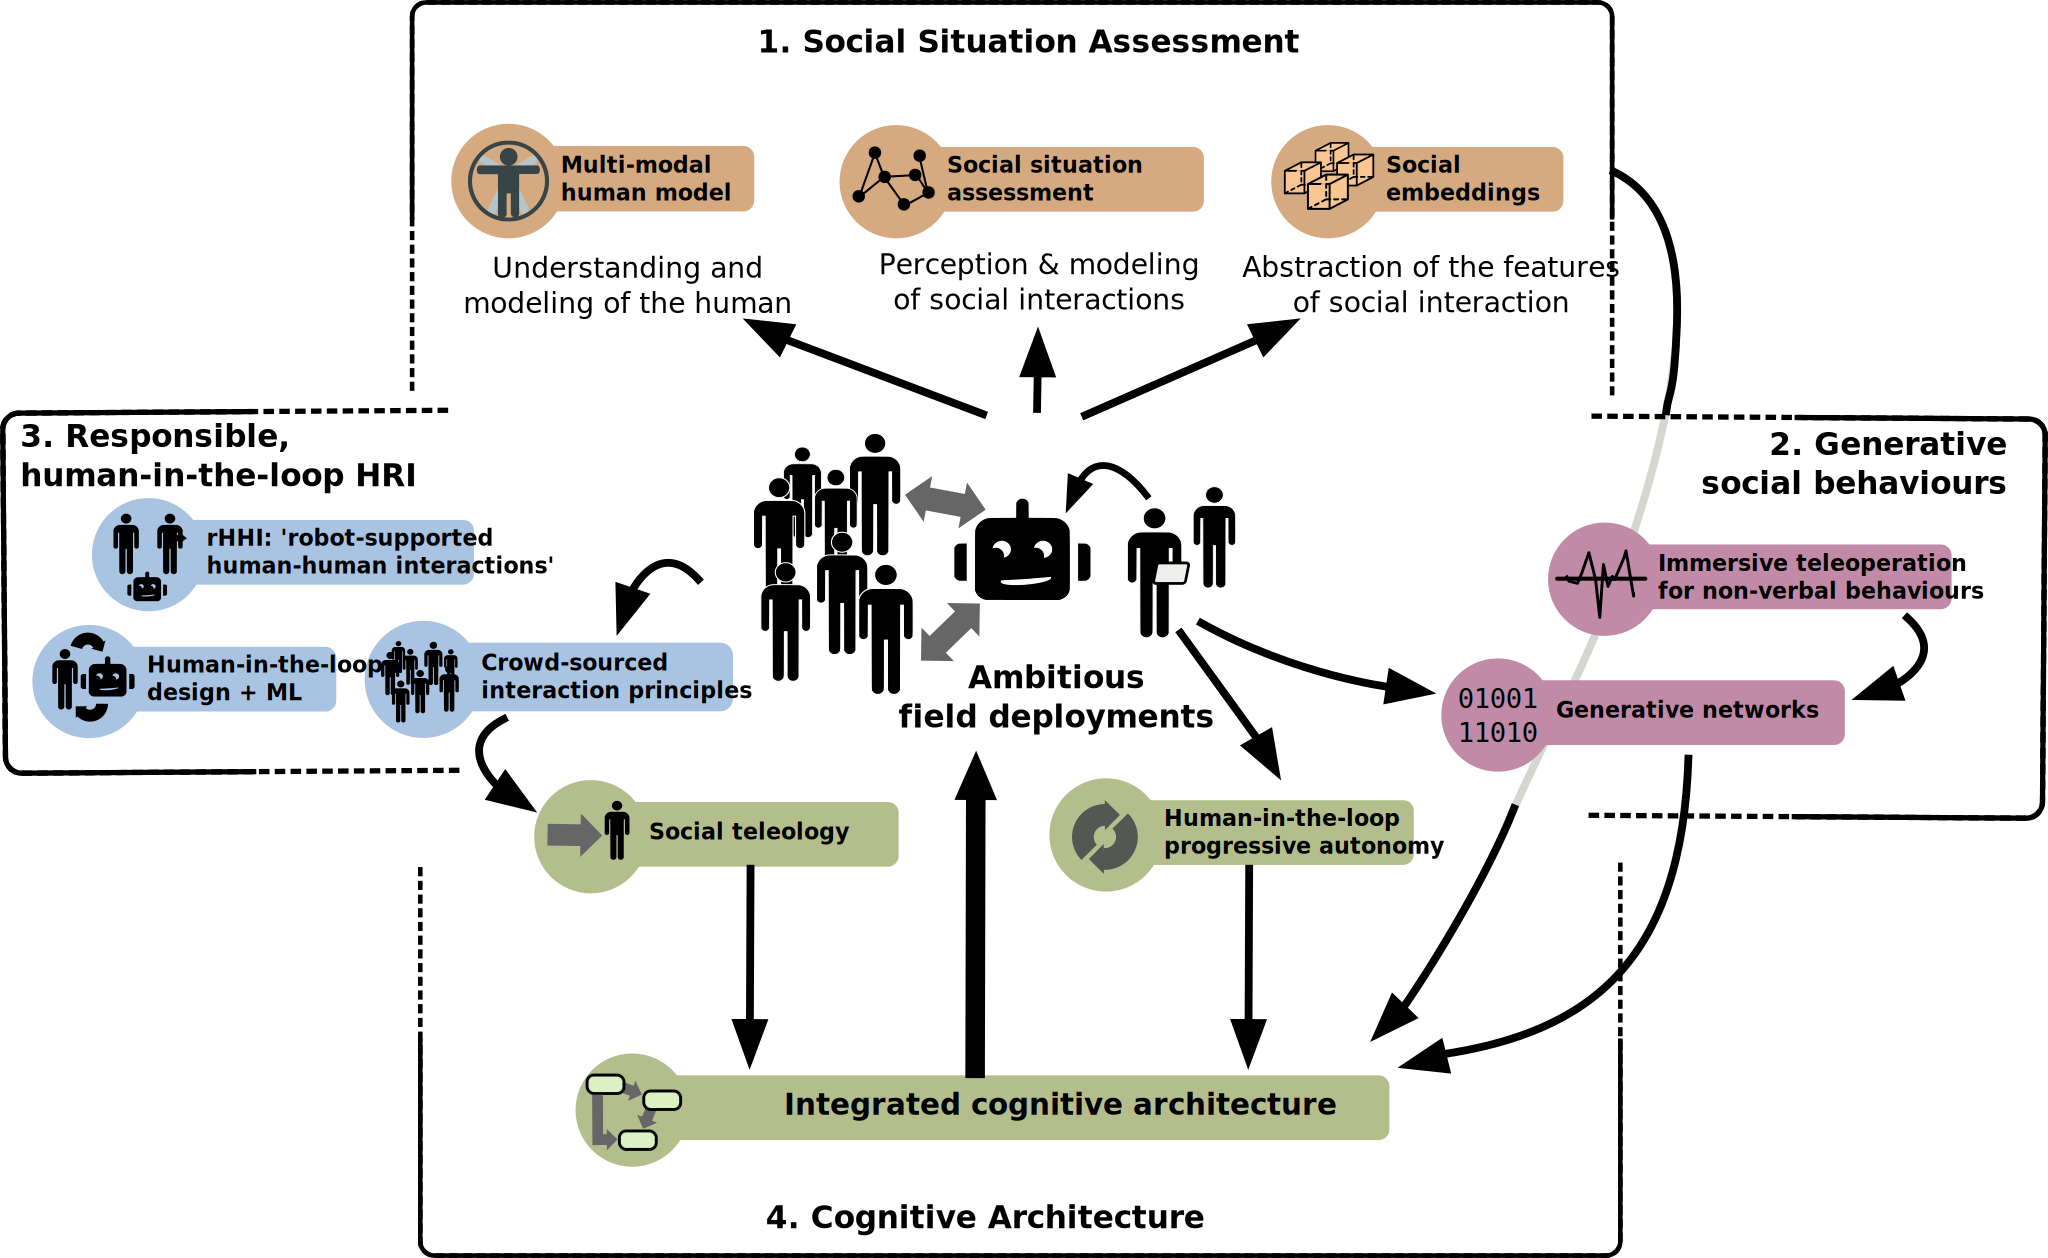
\includegraphics[trim=8cm 0 8cm 16cm,clip,width=\linewidth]{architectures/wps}
    }
    \only<5>{
        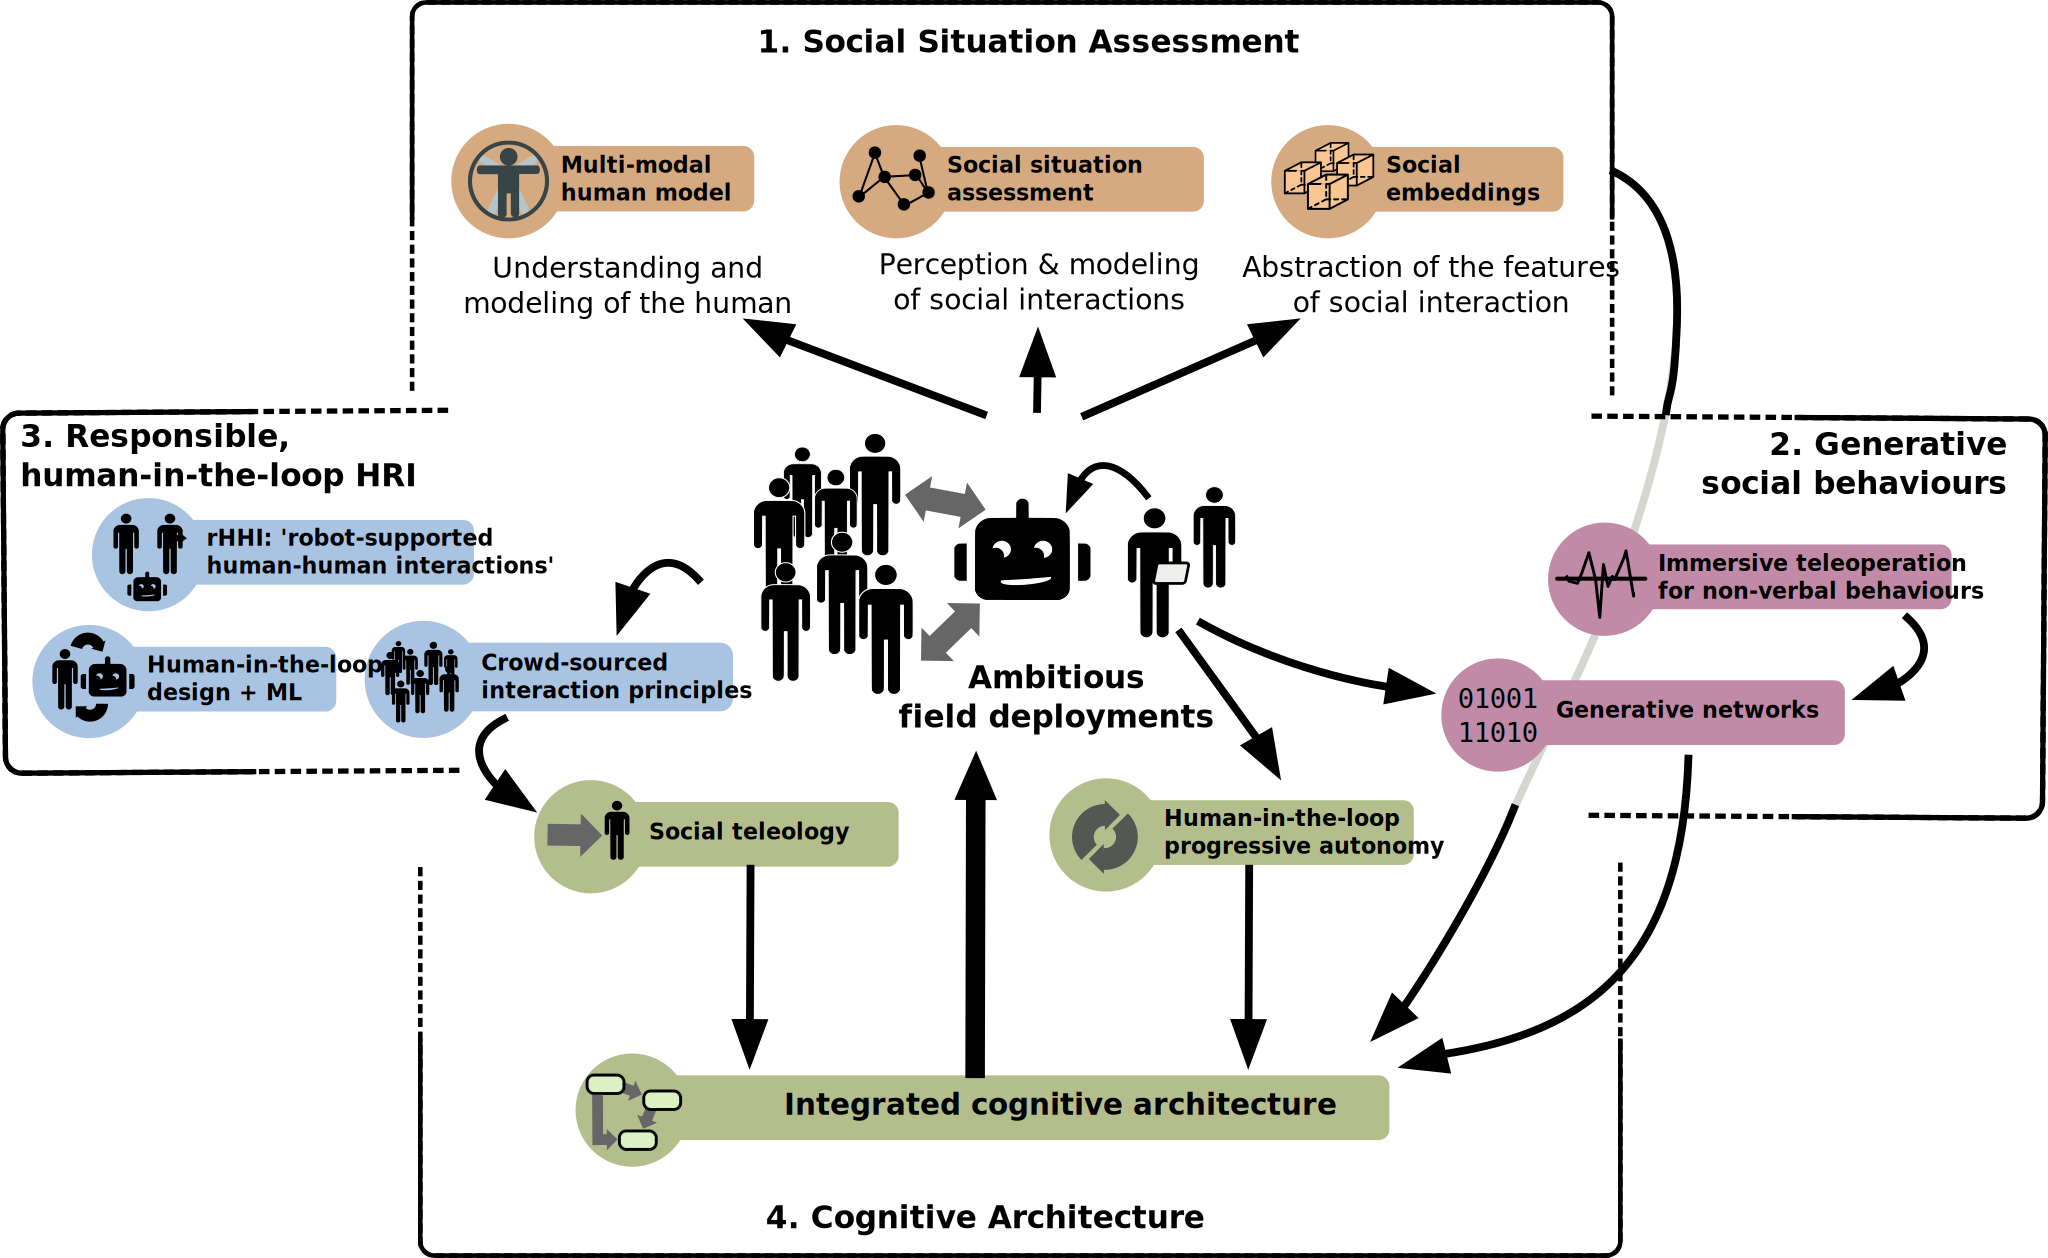
\includegraphics[trim=0 8cm 34cm 8cm,clip,width=0.7\linewidth]{architectures/wps}
    }
    \end{center}
\end{frame}

\begin{frame}{2022: EU ICT bid}
    \begin{center}
        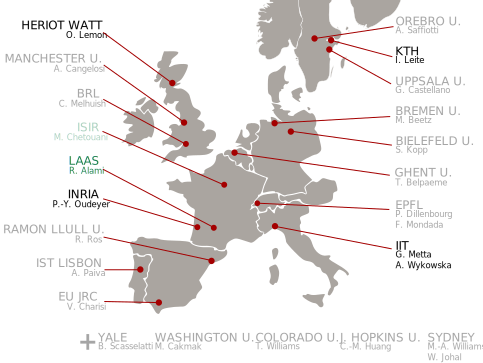
\includegraphics[width=0.8\linewidth]{collaborations_map_project}
    \end{center}
\end{frame}

\miniframesoff{}

\begin{frame}{INTEGRATION LAAS}

    \begin{center}
        
\includegraphics[width=0.3\linewidth]{Laas-CNRS}

    \end{center}

    \begin{itemize}
        \item Long-standing expertise in autonomous social robots (R. Alami) $\rightarrow$ natural integration to RIS team
        \item Excellent infrastructure \& access to robots
        \item Software engineering expertise almost unique in academia
        \item ANITI: Excellent academic environment \& collaboration
            opportunities
    \end{itemize}

    \pause

    \textbf{What I would bring:}

    \begin{itemize}
        \item Experimental know-how with extensive expertise in real-world deployments
        \item Emerging theme: Data-driven HRI
        \item ANITI: transverse applications for AI and robotics
    \end{itemize}
\end{frame}

%%%%%%%%%%%%%%%%%%%%%%%%%%%%%%%%%%%%%%%%%%%%%%%%%%%%%%%%

{
    \fullbackground[color=black]{lastpage}
    \begin{frame}[plain]

        \begin{columns}
            \begin{column}{0.6\linewidth}
            \end{column}
            \begin{column}{0.4\linewidth}

                \setbeamercolor{hriSec1Demo}{fg=white!70!black}
                \vspace{6em}
                \begin{beamercolorbox}[wd=\linewidth,ht=6ex,dp=0.7ex]{hriSec1Demo}
                    \textbf{Thank you!}
                \end{beamercolorbox}
                \vspace{12em}
                {\scriptsize
                \textcolor{white!60!black}{\emph{(photo of 
                \textsc{roboscopie}, a theatre play I created with director Nicolas Darrot in
                2012)}}
                }
            \end{column}
        \end{columns}
    \end{frame}
}

\end{document}
